\documentclass{sig-alternate-05-2015}

% Fix to revert the changes IEEEtran makes to table caption styles
\usepackage{etoolbox}
\makeatletter
\patchcmd{\@makecaption}
  {\scshape}
  {}
  {}
  {}
\makeatother

%===========================================================================
\usepackage{listings}
\lstloadlanguages{C++}

% Settings for the lstlistings environment
\lstset{
language=C++,                       % choose the language of the code
basicstyle=\footnotesize\ttfamily,  % the size of the fonts that are used for the
                                    % code
numbers=none,                       % where to put the line-numbers
numberstyle=\tiny,                  % the size of the fonts that are used for the
                                    % line-numbers
stepnumber=1,                       % the step between two line-numbers. If it's
                                    % 1 each line will be numbered
numbersep=5pt,                      % how far the line-numbers are from the code
%backgroundcolor=\color{gray},      % choose the background color. You must add
                                    % \usepackage{color}
showspaces=false,                   % show spaces adding particular underscores
showstringspaces=false,             % underline spaces within strings
showtabs=false,                     % show tabs within strings adding particular
                                    % underscores
keywordstyle=\bfseries\color{blue},  % color of the keywords
commentstyle=\color{darkgreen},     % color of the comments
stringstyle=\color{darkred},        % color of strings
captionpos=b,                       % sets the caption-position to top
tabsize=2,                          % sets default tabsize to 2 spaces
frame=tb,                           % adds a frame around the code
breaklines=true,                    % sets automatic line breaking
breakatwhitespace=false,            % sets if automatic breaks should only happen
                                    % at whitespace
escapechar=\%,                      % toggles between regular LaTeX and listing
belowskip=0.3cm,                    % vspace after listing
morecomment=[s][\bfseries\color{blue}]{struct}{\ },
morecomment=[s][\bfseries\color{blue}]{class}{\ },
morecomment=[s][\bfseries\color{blue}]{public:}{\ },
morecomment=[s][\bfseries\color{blue}]{public}{\ },
morecomment=[s][\bfseries\color{blue}]{protected:}{\ },
morecomment=[s][\bfseries\color{blue}]{private:}{\ },
morecomment=[s][\bfseries\color{black}]{operator+}{\ },
xleftmargin=0.1cm,
%xrightmargin=0.1cm,
}

\usepackage{color}
\usepackage{comment}
\usepackage{graphicx}
\usepackage{subfig}
\usepackage{multirow}

\usepackage{rotating}
\usepackage{pdflscape}

\captionsetup[subfigure]{position=top}

%\usepackage[font=scriptsize,justification=justified,singlelinecheck=false]{caption}

\usepackage{amsmath}
\usepackage{amsfonts}
\usepackage[hidelinks]{hyperref}
\usepackage{cite}

\usepackage{fixme}
\fxusetheme{color}
\fxsetup{
    status=draft,
    author=,
    layout=inline, % also try footnote or pdfnote
    theme=color
}

\pagenumbering{arabic}

\linespread{2}

%===========================================================================
\begin{document}
\title{Solving Large Quantities of Small Matrix Problems on Cache-Coherent SIMD Architectures}

%===========================================================================
% author names and affiliations
% use a multiple column layout for up to three different
% affiliations
\numberofauthors{1}
\author{
\alignauthor
Bryce Adelstein Lelbach, Hans Johansen, and Samuel Williams\\
\affaddr{Lawrence Berkeley National Laboratory, Computational Research Division}\\
\email{{\it \{balelbach, hjohansen, swwilliams\}@lbl.gov}}
}
% \IEEEauthorblockN{Bryce Adelstein Lelbach, Hans Johansen, and Samuel Williams}
% \IEEEauthorblockA{Computational Research Division, Lawrence Berkeley National Laboratory, Berkeley, CA 94720\\ {\it \{balelbach, hjohansen, swwilliams\}@lbl.gov}}
%\and
%\IEEEauthorblockN{Homer Simpson}
%\IEEEauthorblockA{Twentieth Century Fox\\
%Springfield, USA\\
%Email: homer@thesimpsons.com}
% }

% conference papers do not typically use \thanks and this command
% is locked out in conference mode. If really needed, such as for
% the acknowledgment of grants, issue a \IEEEoverridecommandlockouts
% after \documentclass

% for over three affiliations, or if they all won't fit within the width
% of the page, use this alternative format:
% 
%\author{\IEEEauthorblockN{Michael Shell\IEEEauthorrefmark{1},
%Homer Simpson\IEEEauthorrefmark{2},
%James Kirk\IEEEauthorrefmark{3}, 
%Montgomery Scott\IEEEauthorrefmark{3} and
%Eldon Tyrell\IEEEauthorrefmark{4}}
%\IEEEauthorblockA{\IEEEauthorrefmark{1}School of Electrical and Computer Engineering\\
%Georgia Institute of Technology,
%Atlanta, Georgia 30332--0250\\ Email: see http://www.michaelshell.org/contact.html}
%\IEEEauthorblockA{\IEEEauthorrefmark{2}Twentieth Century Fox, Springfield, USA\\
%Email: homer@thesimpsons.com}
%\IEEEauthorblockA{\IEEEauthorrefmark{3}Starfleet Academy, San Francisco, California 96678-2391\\
%Telephone: (800) 555--1212, Fax: (888) 555--1212}
%\IEEEauthorblockA{\IEEEauthorrefmark{4}Tyrell Inc., 123 Replicant Street, Los Angeles, California 90210--4321}}




% use for special paper notices
%\IEEEspecialpapernotice{(Invited Paper)}




% make the title area
\maketitle

%===========================================================================

\begin{abstract}
A number of computational science algorithms lead to discretizations
  that require a large number of independent, small matrix solves.
Examples include small non-linear coupled chemistry and flow systems,
  one-dimensional sub-systems in climate and diffusion simulations, 
  alternating direction implicit pre-conditioners, and 
  semi-implicit time integrators, among others.
We present a performant approach for solving large quantities of 
  independent matrix problems on cache-coherent SIMD architectures. 
Unlike many vectorized or ``batched'' approaches that rely on reusing
  the matrix factorization across multiple solves, our algorithm supports
  the case of sets of matrices that are different, due to
  spatial variation or non-linear solvers, for example.
We demonstrate the approach with a prototypical tridiagonal matrix solver,
  derived from a 1D solver that is part of an implicit-explicit 
  finite difference discretization for a 3D advection-diffusion problem.
Performance is evaluated on several Intel architectures with different cache,
  vectorization, and threading features, and compared to theoretical
  roofline models across parameter studies.
We conclude that the approach is effective at optimizing both vectorization 
  and memory bandwidth, and improves on existing approaches for efficiently
  solving large numbers of small matrix problems.
\end{abstract}

% no keywords


% For peer review papers, you can put extra information on the cover
% page as needed:
% \ifCLASSOPTIONpeerreview
% \begin{center} \bfseries EDICS Category: 3-BBND \end{center}
% \fi
%
% For peerreview papers, this IEEEtran command inserts a page break and
% creates the second title. It will be ignored for other modes.
% \IEEEpeerreviewmaketitle

%===========================================================================
\section{Introduction}
\label{sec:introduction}

One important class of problems in computational science is the solving
  of smaller-dimensional matrix subproblems that are duplicated across
  many degrees of freedom in a larger two (or more) dimension computation.
Several examples of this include: 
\begin{itemize}
\item Pointwise chemistry systems in the context of a larger, 
  flow simulations. 
Examples include geochemistry~\cite{PFLOTRAN_2010}, 
  cloud microphysics~\cite{MG2_2015}, and combustion~\cite{PaznerEtAl_2016};
\item Solving one-dimensional systems that represent a numerically ``stiff''
  direction for a physical phenomenon.
Examples here include atmospheric radiation~\cite{RRTMG_2008}, groundwater
  penetration~\cite{CLM_PFLO_2016}, or models for 
  cloud convection~\cite{SAM_2005}; and
\item Implicit solvers that need to couple these kinds of subsystems, 
  such as line relaxation~\cite{TrottenbergEtAl_2000} and 
  semi-implicit time integrators~\cite{WellerEtAl_2013}.
\end{itemize}
In most cases, these matrices are relatively small 
  (ranging from \(O(10-100)\) chemistry components or ``levels'' 
  in a climate application), and may be sparse or dense, but must 
  be solved repeatedly, but with different entries each time, 
  to advance the overall simulation.
Thus, because these are often non-linear matrix systems with space- and 
  time-dependent entries, these applications may not use a 
  ``factor once, solve many times'' approach, which is often used 
  as a model matrix performance test.
This prevents amortizing setup and factorization costs
  across multiple right-hand side solves as in 
  \lstinline{dgtsv()}~\cite{IntelMKL_DGTSV} and \lstinline{dgttrs()}~\cite{IntelMKL_DGTTRS},
  and also challenges vectorization due to the odd size and
  dissimilar entries of the matrices, as well as the 
  memory access patterns relative to the bigger simulation data layout.
In that case, it is usually sub-optimal on SIMD many-core or SIMT GPGPU
  architectures to simply call an optimized linear algebra library, 
  such as Intel's Math Kernel Library (MKL)~\cite{mkl_website} or NVIDIA's
  CUDA Basic Linear Algebra Subroutines (cuBLAS)~\cite{cublas_website}; these
  may not achieve peak memory bandwidth and floating-point performance across 
  the range of small matrix size. 
In that sense, it can leads applications to create their own 
  custom implementations, which may not be optimal, and create a 
  (potentially unnecessary) maintenance burden for the applications 
  running across multiple many-core architectures as well. 
  
To this end, we have developed a model matrix kernel that mimics what
  is encountered in these kinds of large-scale simulations.
Key aspects of the code include:
\begin{itemize}
\item A three-dimensional application (that is, \((i,j,k)\) indices),
  where different matrix systems in the \emph{vertical} dimension \(k\) are
  generated at each \emph{horizontal} dimension \((i,j)\). 
\item Each matrix is tri-diagonal, and must be solved for all 
  \(nk \sim O(30-100)\) values in the \(k\) direction.
\item The matrix is derived from finite difference discretization for the
  1D diffusion equation, which allows it to be solved \emph{without pivoting}.
\end{itemize}
We note that pivoting and sparsity patterns are often application-specific;
  these requirements will be addressed in future work.

%===========================================================================
\section{Related Work}
\label{sec:related_work}

%{\color{red} TRIM AND MERGE UP \\
Approaches to solving large numbers of small matrices have been done
  in a variety of contexts.
Many implementations simply solve each matrix in parallel or for multiple
  right-hand sides, using platform-specific
  implementations of LAPACK, such as Intel's MKL or NVIDIA's cuBLAS implementations.
In many cases, there is a benefit from vectorization and thread parallelism, 
  but there may be overheads that reduce performance, such as data copies/
  temporary variables, 
  dynamic determination of optimal performance parameters, 
  and partially vectorized ``peel'' loops, for example.
Some specialized approaches include linear algebra-specific 
  compilers for small problem sizes and target architectures 
 ~\cite{Spampinato:2014, NelsonEtAl_2015}.
Other libraries like 
  \emph{Blaze}~\cite{BlazeSite}, 
  \emph{PLASMA}~\cite{PLASMASite},
  \emph{MAGMA}~\cite{Haidar:2015}, and 
  \emph{libxsmm}~\cite{libxsmm_website}
  are intended to support SIMD vectorization for standard vector sizes
  as well as batched computation for sparse and dense matrices.
Overall, there is a gap in approaches that have both effective vectorization,
  regardless of matrix size, with or without dense/sparse/pivoting 
  assumptions, amortizing factorization across multiple right-hand-sides, 
  and other assumptions.
%}
%===========================================================================
\section{Implementation}
\label{sec:implementation}

Suppose we have an \(nk \times nk\) tridiagonal matrix \(A\) and two \(nk\) element
  vectors \(u^{s}\) and \(u^{s+1}\).  We wish to solve \(Au^{s+1} = u^{s}\) for
  \(u^{s}\):
\fxnote[footnote,noinline]{Bryce: I'd like to say symmetric positive-definite
  or diagonally-dominant here to make it clear that our solver only works with
  certain classes of tridiagonal matrices.}

\[
\begin{bmatrix}
b_0 & c_0 &     &          & 0        \\
a_1 & b_1 & c_1 &          &          \\
    & a_2 & b_2 & ...      &          \\
    &     & ... & ...      & c_{nk-2} \\
0   &     &     & a_{nk-1} & b_{nk-1}
\end{bmatrix}
\begin{bmatrix}
u^{s+1}_0     \\
u^{s+1}_1     \\
...     \\
...     \\
u^{s+1}_{n-1}
\end{bmatrix}
=
\begin{bmatrix}
u^{s}_0     \\
u^{s}_1     \\
...     \\
...     \\
u^{s}_{n-1}
\end{bmatrix}
\]

Our matrix \(A\) is stored as a set of three vectors: an \(nk-1\) element
  sub-diagonal vector \(a\), an \(nk\) element diagonal vector \(b\) and an
  \(nk-1\) element super-diagonal vector \(c\).
In practical applications, a different matrix \(A\) exists for each \((i,j)\)
  location, because the diagonals may depend on the previous solution \(u^{s}\)
  (in a non-linear iteration loop, for example).

\fxnote{Paragraph overview of SSTA solver}

\subsection{The Thomas Algorithm}
\label{sec:implementation:thomas_algorithm}

For a \emph{diagonally-dominant} tridiagonal matrix, we can use a simplified
  form of Gaussian elimination that does not require pivoting, known as the
  Thomas algorithm or the tridiagonal matrix algorithm
  (TDMA)~\cite{ConteEtAlElementaryNumericalAnalysis,QuarteroniEtAl2007,TDMA}. 
This takes advantage of sparsity to be \(O(nk)\) in time, 
  and can be extended to banded matrices and LU factorizations.
It is also a significant improvement over dense Gaussian elimination,
  which is \(O(nk^3)\) in time. 
We use a formulation of the Thomas algorithm which does not require any storage
  for temporary values but overwrites the \(b\) vector and solves for \(u^{s+1}\)
  in-place, overwriting \(u^{s}\).

The Thomas algorithm consists of two passes.  First, a forward pass is
  performed to eliminate the \(a_i\) elements:
\begin{lstlisting}
for (auto k = 1; k < nk; ++k) {
  auto const m = a[k] / b[k - 1];
  b[k] -= m * c[k - 1];
  u[k] -= m * u[k - 1];
} 
\end{lstlisting}
Then, an abbreviated form of backwards substitution is performed to obtain the
  solution:
\begin{lstlisting}
u[nk - 1] = u[nk - 1] / b[nk - 1];

for (auto k = nk - 2 ; k >= 0; --k) {
  u[k] = (u[k] - c[k] * u[k + 1]) / b[k];
} 
\end{lstlisting}

The Thomas algorithm is a very low algorithmic intensity (AI)~\cite{roofline}
  algorithm.
During the course of our work, we developed a theoretical peak performance
  model for the Thomas algorithm.
First, we count the number of FLOPs performed.
We will consider multiplications, additions and division operations as FLOPs.

Each iteration of the forward elimination loop contains 1 division, 2
  multiplications and 2 subtractions.
This gives us a total of either \(3(nk-1)\) FLOPs on fused-multiply-add (FMA)
  architectures~\cite{} or \(5(nk-1)\) FLOPs on non-FMA architectures.
Next, the pre-substitution operation (the assignment to \lstinline{u[nk - 1]}
  in the above snipper) performs a single division.
Finally, the backwards substitution loop, performs 1 multiplication, 1
  subtraction and 1 division, adding either \(2(nk-1)\) FLOPs (FMA architectures)
  or \(3(nk-1\) FLOPs (non-FMA architectures).
In total, this gives us either \(5nk-4\) FLOPs (FMA) or \(8nk-7\) FLOPs
  (non-FMA) for the entire Thomas algorithm.

Our data movement model for the Thomas algorithm assumes that we will achieve
  optimal performance when data is cached between the forward elimination and
  back substitution loop.
That is, we assume that accesses to \(a\), \(b\), \(c\) and \(u\) will
  \emph{not} go to main memory in the back substitution loop because the arrays
  still remain in cache from the forward elimination loop accesses.

The Thomas algorithm accesses four arrays, reading from all of them (\(a\),
  \(b\), \(c\) and \(u\)) and writing to two of them (\(b\), \(u\)).
\(b\) and \(u\) have extent \(nk\), so we write \(2nk\) elements.
\(a\) and \(c\) have extent \(nk-1\), so we read \(2(nk-1)+2(nk)\) elements.
In total, \(6nk-2\) elements are moved.
Assuming double precision, \(48nk-16\) bytes are moved from main memory
  during execution of the Thomas algorithm.

This gives us a FLOPs/byte ratio of \((5nk-4)/(48nk-16)\) (FMA) or
  \((8nk-7)/(48nk-16)\) (non-FMA).
The lower bound for the Thomas algorithm's arithmetic intensity is \(1/32\)
  FLOPs/byte when \(nk=1\). 
The upper bound is \(5/48\) FLOPS/byte (FMA) or \(1/6\) FLOPs/byte (non-FMA) as
  \(nk\) approaches infinity.
Based on this analytic analysis, we can conclude that the Thomas algorithm is
\emph{memory-bandwidth bound}.

%In each iteration of the forward elimination loop, we perform 1 division, 2
%multiplications and 2 subtractions. The multiplications and subtractions will
%be performed as a single fused-multiply-adds (FMA) instructions on supported
%platforms. For now, we will treat naively count division operations as a single
%FLOP. Thus, the forward elimination pass will require either 3 FLOPs or 5 FLOPs
%per iteration, or a total of either \(3(nk-1)\) FLOPs (on FMA architectures) or
%\(5(nk-1)\) FLOPs (on non-FMA architectures). The pre-substitution operation
%(the assignment to \lstinline{u[n - 1]} in the above snipper) performs a single
%division, adding 1 FLOP to the total count. Finally, we have the backwards
%substitution loop, which performs 1 multiplication, 1 subtraction and 1
%division. This adds either 2 FLOPs or 3 FLOPs, or a total of either \(2(nk-1)\)
%FLOPs (FMA) or \(3(nk-1\) FLOPs (non-FMA). Summing all the counts up, this
%gives us either \(3(nk-1)+2(nk-1)+1=5nk-4\) FLOPs (FMA) or
%\(5(nk-1)+3(nk-1)+1=8nk-7\) FLOPs (non-FMA) for the entire Thomas algorithm.
%
%Now let us consider the amount of data moved from and to main memory during
%execution of the Thomas algorithm.  We assume that we will achieve optimal
%performance when data which has been previously loaded does not need to be
%reloaded from main memory. We assume that accesses of elements from previous
%iterations will be loaded from a cache, not main memory (\lstinline{u[n - 1]}
%in the backward substitution loop for example). Our performance model also make
%the stronger assumption that the arrays \(a\), \(b\), \(c\) and \(u\) will be
%cached in between the forward elimination loop and the back substitution loop.
%
%{\color{red} CUT, FIX FOR FLOW \\
%Thus, we take a more macro approach to counting data movement. The algorithm
%accesses four arrays, reading from all of them and writing to two of them
%(\(b\), \(u\)). Two of the arrays have extent \(nk-1\), and have extent \(nk\).
%Thus, we read \(2(nk-1)+2(nk)=4nk-2\) elements. The arrays which we write to
%have extent \(nk\), so we write \(2nk\) elements. In total, \(2nk+4nk-2=6nk-2\)
%elements are moved. Assuming double precision, this means
%\((6nk-2)\)\lstinline{sizeof(double)}\(=48nk-16\) bytes are moved from main
%memory during the execution of the Thomas Algorithm.
%}
%
%This gives us a FLOPs/byte ratio of \((5nk-4)/(48nk-16)\) (FMA) or
%\((8nk-7)/(48nk-16)\) (non-FMA). The lower bound for the Thomas algorithm's AI
%is \(1/32\) FLOPs/byte (for both FMA and non-FMA architectures) when \(nk=1\)
%(which is, of course, a nonsensical problem size). The upper bound (e.g. the
%limit as \(nk\) approaches infinity) is \(5/48\) FLOPS/byte (FMA) or \(1/6\)
%FLOPs/byte (non-FMA).

%Although some of the optimizations described in this paper slightly increase the
%ratio (e.g. the division optimizations described in \S\ref{sec:divopt}), 
%the order of magnitude does not change.

%\subsection{Division Optimizations}
%\label{sec:implementation:division_optimizations}
%
%% 1st Reference here is Intel Optimization Manual, 11.12
%% 2nd Reference here is the intrinsic manual
%When we analyzed implementations of the Thomas algorithm as described above, we
%observed that while the it is primary memory-limited, performance could be
%sensitive to the latency of the floating point divisons present in the
%algorithm. Vectorized floating point operations which use the division
%execution unit (divides, fast reciprocal estimation, square root) are not
%pipelined on many mainstream architectures, including Intel SSE, AVX and AVX2
%platforms~\cite{}. Thus, these operations have very high latency (43 cycles for
%an AVX 256-bit double-precision divide on Sandy Bridge; 35 cycles on Ivy Bridge
%and Haswell~\cite{}) and low throughput relative to other floating point
%operations such as multiplication and addition.
%
%%Variants of the TDMA algorithm have been developed to minimize 
%%divides~\cite{QuarteroniEtAl2007} by caching them in temporary variables.
%%Our approach is to compute and store temporary reciprocal values in the
%%diagonal vector \(b\), which removes the division in the backwards 
%%substitution pass.
%
%In the in-place Thomas algorithm described above, all the division operations
%have the same divisor - the temporary coefficient computed and stored in the
%diagonal vector b. If we re-formulate the algorithm to store the reciprocal of
%that coefficient instead of storing the coefficient itself, we are able to
%replace the division in the backwards substitution pass with a multiplication.
%We call this the \textbf{cached-divide} in-place TDMA algorithm. The forward
%elimination pass becomes:
%
%\begin{lstlisting}
%b[0] = 1.0 / b[0];
%
%for (auto k = 1; k < n; ++k) {
%  auto const m = a[k] * b[k - 1];
%  b[k] = 1.0 / (b[k] - m * c[k - 1]);
%  u[k] = u[k] - m * u[k - 1];
%} 
%\end{lstlisting}
%
%The backwards substitution pass becomes:
%
%\begin{lstlisting}
%u[n - 1] = u[n - 1] * b[n - 1];
%
%for (auto k = n - 2 ; k >= 0; --k) {
%  u[k] = (u[k] - c[k] * u[k + 1]) * b[k];
%} 
%\end{lstlisting}
%
%% Could have said more here.
%This optimization slightly increases the number of FLOPs performed by the
%Thomas algorithm, although the amount of data movement remains unchanged.
%
%{\color{red} CUT AGGRESSIVELY, JUST LEAVE A LITTLE ALGO DESCRIPTION \\
%One well-known technique for optimizing floating point divisions is to replace
%division operations with fast reciprocal estimates (RCP) when possible. On many
%platforms where floating point division operations are not pipelined, floating
%point RCP operations will also not be pipelined, however they generally have
%much lower latency and higher throughput than division operations. Many
%optimizing compilers will transparently and reliable perform this optimization.
%However, there is a caveat on 256-bit AVX and AVX2 platforms (e.g. Sandybridge,
%Ivy Bridge, Haswell and Skylake); no double-precision RCP is available on these
%platforms, although a single-precision RCP instruction is available.
%
%We experimented with the use of a single-precision RCP and Newton Raphson
%iteration to compute a fast division estimation. We are not aware of a compiler
%which provides optionally provides this optimization. To implement the
%optimization, we simply type cast the double-precision values to
%single-precision, perform a division operation, cast back to double-precision
%and then preform Newton Raphson iterations (at double precision). We rely on
%the compiler to replace the division with an RCP instruction.
%
%\begin{lstlisting}
%template <std::size_t NRIterations = 1>
%double nr_rcp_divide(double num, double den) {
%  double x = float(1.0) / float(den);
%
%  for (auto i = 0; i < NRIterations; ++i)
%    x = x + x * (1.0 - den * x);
%
%  return num * x;
%}
%\end{lstlisting}
%
%Since the single-precision RCP instruction will operate on twice as many values
%as a double-precision division from the same instruction set, when our division
%estimate is used in a vectorized loop it is prudent to unroll the loop at least
%once so that one single-precision RCP instruction can service two
%double-precision iterations. Again, we have been able to rely on the compiler
%to handle this component of the optimization.
%
%We do pay an overhead for the type conversion, in the form of packed-double to
%packed-single vector instructions as well as additional double-precision
%multiplications and additions. There is also an accuracy trade-off, however,
%with a single Newton Raphson iteration, we observed an L2 norm and maximum
%residual with the same order of magnitude as the variant of our code which uses
%division instructions.
%}
%
%We found this optimization to be beneficial when executing in serial on a
%single processing unit. Our results from parallel runs indicate that we can not
%statistically distinguish any impact from this optimization when running in
%parallel. We did find that, both in serial and in parallel, the RCPPS
%optimization had a negative effect when combined with the cached-divide
%optimization. See Section \ref{} and Figure \ref{} for further discussion of
%these results.

\subsection{Batching and Vectorization}
\label{sec:implementation:batching_and_parallelism}

\begin{figure}[!bt]
  \centering
  \label{fig:independent_solve_strategy}
  \caption{
    \textbf{Independent Solve Strategy:} \fxnote{Lorem Ipsum}
  }
  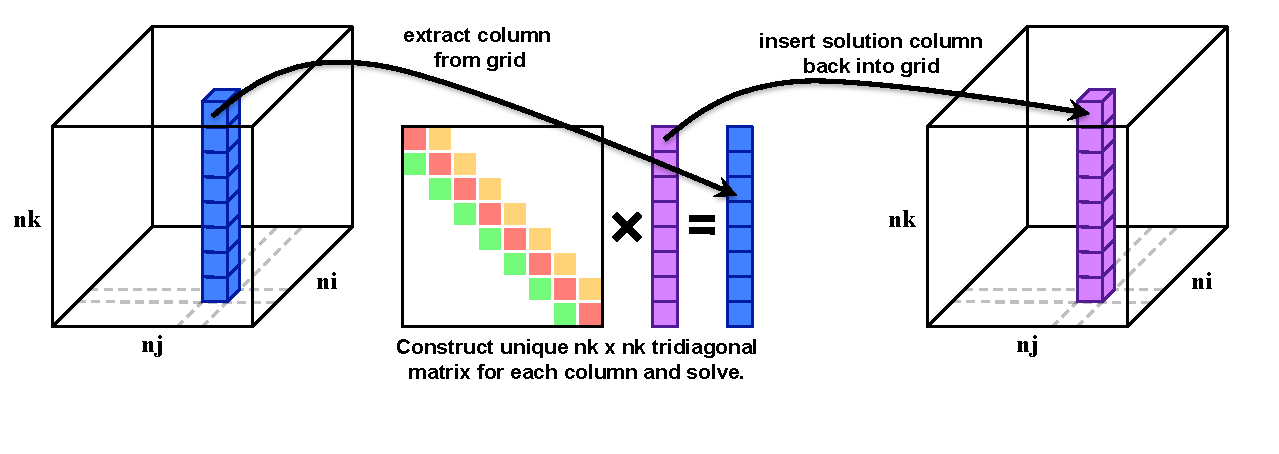
\includegraphics[width=0.95\columnwidth]{figures/tds_scalar.pdf}
\end{figure}

\begin{figure}[!bt]
  \centering
  \label{fig:simultaneous_solve_strategy}
  \caption{
    \textbf{Simultaneous Solve Strategy:} \fxnote{Lorem Ipsum}
  }
  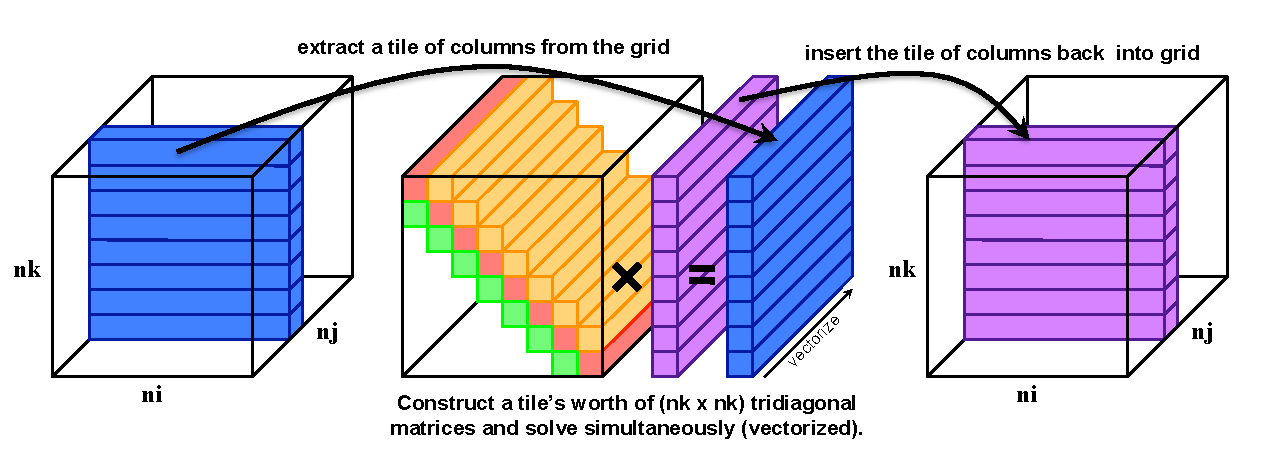
\includegraphics[width=0.95\columnwidth]{figures/tds_vector.pdf}
\end{figure}

In the applications described in \S\ref{sec:introduction} we need to apply the
  Thomas algorithm to each vertical column in a \(ni \times nj \times nk\)
  Cartesian grid, where \(i\) and \(j\) are horizontal dimensions and \(k\) is
  the vertical index.
These computations are known as the \emph{vertical solves}.
The matrix coefficients for each column depend on the problem state, so a
  unique matrix for each column needs to be constructed before each solve.
There are two different approaches to computing these batch solves.

The most straightforward approach is \emph{solve} each column
  \emph{independently} (the \emph{independent solve strategy}; Figure
  \ref{fig:implementation:independent_solve_strategy}).
An \(nk \times nk\) tridiagonal matrix is constructed for each column, and then
  the Thomas algorithm is used to solve the system formed by the matrix and the
  vertical column.
Because the vertical solves are independent, they can be executed concurrently
  via task-level parallelism.
Vectorization of the \(nk\) loop is not possible as each iteration of the loops
  in the Thomas algorithm is dependent on the previous iteration (e.g.
  loop-carried dependency).
Although the LAPACK interface contains no routine for Thomas algorithm,
  \lstinline{dgtsv()} and \lstinline{dgttrs()} (which solve tridiagonal and
  banded systems, respectively) use this approach.

The other approach is to \emph{simultaneously solve} multiple columns (the
  \emph{simultaneous solve strategy}; Figure
  \ref{fig:implementation:simultaneous_solve_strategy}).
A block \(nk \times nk\) tridiagonal matrix is constructed for the whole grid;
  each block contained within the matrix is an \(ni \times nj\) horizontal plane
  (e.g. the block matrix is a 4D space).
To perform the vertical solves, we view the entire 3D Cartesian grid as an
  \(nk\) block vector of \(ni \times nj\) planes and apply it to the block
  matrix.
Each step of the algorithm is applied across an entire plane.
For example, the forward sweep becomes:
\begin{lstlisting}
for (auto k = 1; k < nk; ++k)
for (auto j = 0; j < nj; ++j)
for (auto i = 0; i < ni; ++i) {
  auto const m = a[i][j][k]
               / b[i][j][k - 1];
  b[i][j][k] -= m * c[i][j][k - 1];
  u[i][j][k] -= m * u[i][j][k - 1];
} 
\end{lstlisting}
This approach facilities both task-level parallelism and vectorization.
The grid and block matrix can be tiled into smaller subgrids, and the Thomas
  algorithm can be applied to each subgrid independently.
Each step of the Thomas algorithm can be vectorized across the \(ni \times nj\)
  horizontal plane that it is operating on: e.g. the \(i\) or \(j\) loops in the
  above snippet can be vectorized.
For the SSTA solver, the horizontal dimension \(i\) is always the unit stride
  dimension, and the direction in which we vectorize.

%\fxnote{TODO: Explain that the independent solve approach is what LAPACK does,
%and that's why it is insufficient for this type of problem. Also, explain that
%LAPACK has no routine for Thomas-style tridiagonal solves - dgtsv is
%generalized, does actual Gaussian eliminiation and may do pivoting. Also
%mention somewhere that MKL does not parallelize dgtsv.}

%{\color{red} CUT REDUNDANT WITH INTRO \\
The vector parallelism exposed by the simultaneous approach offers a major
  benefit over the independent approach, since it is not possible to vectorize
  most of the kernels in the independent approach due to data dependencies
  between iterations of the Thomas algorithm.
Even if it was possible to vectorize in the vertical \(nk\) dimension, it would
  still be undesirable to do so.
The extent of the vertical dimension tends to be very small in the applications
  we are concerned with \(O(30-100)\).
Vectorizing in the horizontal dimensions allows us to control locality and loop
  trip counts via tiling.
%}

\subsection{Data Layout}
\label{sec:implementation:data_layout}

The data layout of the Cartesian grid has a huge impact on the performance
  potential of the vertical solves.
Throughout the course of our research, our understanding of the impact of
  different data layouts has evolved substantially.
We have investigated three different schemes:
\begin{table}[h]
\centering
% NOTE: kji AKA column-major, Fortran, left
% NOTE: ijk AKA row-major, C++, right
%\caption{\textbf{Data Layouts for the 3D Cartesian Grid:} The following three
%data layouts were investigated in the course of this research. The \(kji\)-layout
%is optimal for the independent solve strategy. The \(ijk\)-layout is effective
%for the simultaneous solve strategy, but the \(ikj\)-layout provides better
%data locality (\S\ref{lab:tiling}) and out performs the \(ijk\)-layout on
%Knight's Landing (Figure \ref{})}
\caption{\textbf{Data Layouts for the 3D Cartesian Grid}}
\begin{tabular}[t]{|c|c|c|c|} \hline
\textbf{Name}         & \textbf{i-stride} & \textbf{j-stride} & \textbf{k-stride}   \\\cline{2-3}
                      & \multicolumn{2}{|c|}{\textbf{(Horizontal)}}                 & \textbf{(Vertical)} \\ \hline
\(ijk\), Column-Major & \(1\)             & \(ni\)            & \(ni * nj\)         \\ \hline
\(kji\), Row-Major    & \(nj * nk\)       & \(nk\)            & \(1\)               \\ \hline
\(ikj\)               & \(1\)             & \(ni * nz\)       & \(ni\)              \\ \hline
\end{tabular}
\label{tab:implementation:data_layout:layouts}
\end{table}

The production code that our MKL baseline solver is derived from uses the
  \(ijk\)-layout.
The vertical columns that we need to pass in to MKL as the solution vector
  (\(u\)) are non-contiguous, as the vertical dimension \(k\) is the dimension
  with greatest stride.
Currently, the production codebase allocates a temporary gather buffer, copies
  data from the grid into the buffer, calls the LAPACK solver, and then copies
  the result from the buffer back to the grid.

%{\color{red} CUT-MERGE LEARNINGS IN NEXT \S~\ref{sec:tiling} \\
We have found the \(kji\)-layout to be optimal for our MKL baseline solver.
With the \(kji\)-layout, we have contiguous vertical columns which can be
  passed to MKL without temporary allocations or unnecessary copies.
We observed a noticeable performance increase from this change with very
  little source code impact, although we have not studied the impact of this
  layout change on horizontal solver components.

%Eventually, we determined that LAPACK would not be sufficient for the vertical
%solves and that we could achieve substantially higher bandwidths by developing
%the solver described in this paper, we revisited the data layout question. As
%we would not be able to vectorize the Thomas algorithm in the vertical
%dimension due to the the loop-carried dependencies present in the algorithm, we
%decided to switch back to an \(ijk\) layout, where one horizontal dimension (\(i\))
%is the unit stride dimension and the vertical dimension (\(k\)) has the greatest
%stride.

Our SSTA solver uses either the \(ijk\)- or \(ikj\)-layout.
The SSTA algorithm vectorizes in one of the horizontal directions (as described
  in \S\ref{sec:implementation:batching_and_parallelism}), so it is desirable to
  use layouts where the horizontal dimension that we are vectorizing (\(i\)) is
  the unit stride dimension, avoiding strided vector loads.
The \(ikj\) layout arose as an optimization to combat data locality and prefetching
  issues which hindered performance on the Intel Xeon Phi Knight's Landing
  architecture, and is described in greater detail in the following section.
%}

\subsection{Tiling}
\label{sec:implementation:tiling}

To ensure good CPU cache utilization, it is often necessary to break a larger
  grid into smaller \textbf{tiles} which better amortize nested loop overheads, expose
  greater data locality and keep data resident in a particular level of the
  cache hierarchy~\cite{blocked_algorithms}.
This technique is also known as \textbf{cache blocking}.
Additionally, partitioning a grid with dimensions known at application
  initialization into fixed size tiles can provide some of the performance
  benefits of compile-time-fixed dimensions (e.g. compiler optimizations) with
  the flexibility of a dynamically sized problem~\cite{kokkos}.
Tiling also provides a useful abstraction for task parallelization, as
  each tile can be computed independent of other tiles and has no overlapping
  data accesses.
Tiling is particularly important for memory-bandwidth bound computations like
  tridiagonal matrix solves.

The production code which our MKL baseline solver is derived from is not task
  parallelized or explicitly tiled.
Since each column is solved independently, there is little opportunity to improve
  locality and reuse via tiling.
Conceptually, since each column is solved independently in the production code,
  it is \emph{effectively} tiled, albeit with a very small tile size (a single
  column, e.g. \(O(nk) \sim O(30-100)\)).
Our MKL baseline solver is tiled solely to facilitate task parallelization.

On the other hand tiling is very fundamental to our SSTA solver.
Our analytical performance model (\S\ref{sec:implementation:thomas_algorithm})
  is based on caching assumptions which we rely on tiling to enforce.
In particular, we assume that all four arrays (\(a\), \(b\), \(c\) and \(u\))
  to remain in the cache hierarchy in between the forward elimination and the
  back substitution loops.
On x86-64 SIMD architectures, we typically aim to fit within the L2 cache.
If any of these four arrays need to be reloaded from main memory in between the
  forward elimination and back substitution loops, the amount of main memory data
  movement is significantly increased and the algorithmic intensity of the
  algorithm decreases dramatically.
While our untiled SSTA results outperform the MKL baseline results (Figure
  \ref{fig:results:efficiency}), they were well below the manufacturer-specified
  bandwidth and STREAM Triad effective bandwidth.

Because it is necessary for all four arrays to remain in the cache hierarchy, 
  it is important to note the distinction between \textbf{per-array tile size}
  (e.g. the tile size for one of the four arrays) and the
  \textbf{total tile size} (e.g. the sum of the per-array tile sizes).
The total tile size is the amount of data we need to remain in cache in between
  the forward elimination and back substitution loops.

\fxnote{Use total tile size/per-array tile size from this point forward}

Due to the loop-carried dependencies in the Thomas algorithm and the small
  extent of \(nk\), we could not tile the vertical dimension. So, we explored two
  tiling schemes which partition the horizontal space.

%{\color{red} CUT MOST OF DISCUSSION, JUST STATE OPTIONS \\
The \textbf{tile-\(ij\)} scheme partitions both the \(i\) and \(j\) dimensions,
  yielding tiles with arbitrary horizontal shape. 
The \textbf{tile-\(j\)} scheme partitions only the \(j\) dimension, producing
  tiles of containing some of number of complete \(i\) (unit-stride) lines.
There is a trade-off between these two schemes, with the tile-\(ij\) scheme
  offering greater flexibility in tile size and the tile-\(j\) scheme offering
  greater contiguity. 

For example, suppose we partition an \(ijk\)-layout grid into four tiles with
  both the tile-\(ij\) scheme (producing \(ni/2 \times ni/2 \times nk\) tiles)
  and the tile-\(i\) scheme (producing \(ni \times ni/4 \times nk\) tiles).
Both tiles have the same size, \(nk \times ni^2/4\) elements.
However, the tile-\(j\) scheme has much greater data contiguity.
For the tile-\(ij\) scheme, tiles contain are \(nk \times ni/2\) contiguous
  \(i\)-lines, each containing \(ni/2\) elements.
For the tile-\(j\) scheme, tiles contain are \(nk\) contiguous \(ij\)-planes,
  each containing \(ni^2/4\) elements.

While the tile-\(j\) scheme offers greater contiguity than the
  tile-\(ij\) in this example, the tile-\(j\) tiles are not a single contiguous
  memory region.
The only way to obtain completely contiguous tiles in the \(ijk\)-layout would
  be to tile the dimension with the greatest stride (\(k\)), which is not possible
  because we cannot partition the vertical dimension.

This limitation led us to the \(ikj\)-layout for the SSTA solver.
In this layout, the direction of vectorization (\(i\)) is still the unit stride
  dimension, avoiding strided loads and assisting hardware prefetching.
Additionally, the tile-\(j\) tiles are completely contiguous regions of memory,
  decreasing translation-lookaside buffer pressure, increasing locality for
  caching and further assisting hardware prefetching.

Consider switching to the \(ikj\)-layout in the prior example.
The tile-\(ij\) tiles would contain \(ni/2\) contiguous \(ik\)-planes, each
  containing \(nk \times ni/2\) elements.
The tile-\(j\) tiles would be one contiguous region containing
  \(nk \times ni^2/4\) elements.

%We have observed that the greater contiguity of the tile-\(j\) approach leads
%  to fewer strided memory accesses, improved hardware prefetching and fewer
%  translation lookaside buffer (TLB) entries needed per tile (discussed in
%  \S\ref{results} and shown in Figure \ref{ref:results:tile_size_knl} and
%  \ref{ref:results:efficiency}).

The only notable downside to the tile-\(j\) scheme is the loss of
  flexibility in tile sizes.
The smallest tile size for the tile-\(j\) scheme is a \(ni \times 1 \times nk\)
  tile (an \(i\)-line of columns), while the smallest tile size for the
  tile-\(ij\) scheme is a \(1 \times 1 \times z\) tile (a single column).
We have not found this restriction to be overly problematic.
If the extent of \(i\) was large enough that the sum of the minimum tile sizes of
  the arrays \(a\), \(b\), \(c\) and \(u\) was greater than the capacity of the
  cache that we wished to reside within, we could likely switch to the tile-\(ij\)
  scheme without experiencing performance degradation due to decreased locality.

The SSTA solver supports both the \(ijk\)- and \(ikj\)-layout.
The tile-\(j\) scheme is used with both layouts.

%\subsection{Aliasing Conflict Mitigation}
%\label{sec:implementation:cache_aliasing_conflict_mitigation}
%
%In addition to to data layout selection and tiling, it was necessary for us to
%mitigate potential data cache conflicts, to ensure optimal cache performance.
%It is necessary to both align and pad the four arrays used in our solver to
%avoid accessing array elements which have addresses that are structurally
%similar enough to be mapped to the same cache set (e.g. two addresses which are
%aligned to the same power of two).
%
%The loops in our algorithm will always access elements of four different arrays
%with the same horizontal (\(ij\)) indices, and will access at most two
%different adjacent vertical (\(k\)) indices. So, to avoid conflicts we must ensure 
%that:
%
%\begin{itemize}
%\item \textbf{Inter-Array Conflicts} Elements of different arrays which have the same \(ijk\) indices map to different cache sets.
%\item \textbf{Vertical Conflict} Elements of the same array which share the same \(ij\) indices map to different cache sets.
%\end{itemize}
%
%
%{\color{red} SIMPLIFY / CONDENSE, MOVE DETAILS TO APPENDIX/README \\
%As described in the previous section, we expected the optimal tile size for
%NAMEFORALGO to be small enough to fit into the L2 cache, so our cache conflict
%considerations only account for L1D and L2 cache conflict misses. Note the
%formula for the size of a set-associative cache (brackets denote units):
%
%\begin{table*}[t]
%\centering
%\caption{\textbf{Formulae for Cache Conflict Mitigation Parameters:}}
%
%\begin{align*}
%CacheSize \: \text{[Bytes]} = Associativity \: \text{[Ways]} * CacheLineSize \: \text{[Bytes]} * NumberOfSets \: \text{[Sets]}
%\end{align*}
%
%\begin{align*}
%BytesPerWay \: \text{[Bytes / Way]} = CacheSize \: \text{[Bytes]} / Associativity \: \text{[Ways]}
%\end{align*}
%
%\begin{align*}
%L1DArrayAlignStep \: \text{[Bytes]} &= L1DBytesPerWay \: \text{[Bytes / Way]} \: / \: 4 \: \text{[Arrays]} \\
%L2ArrayAlignStep \: \text{[Bytes]}  &= L2BytesPerWay \: \text{[Bytes / Way]}  \: / \: 4 \: \text{[Arrays]} \\ 
%ArrayAlignStep \: \text{[Bytes]}    &= L1DArrayAlignStep \: \text{[Bytes]} + L2ArrayAlignStep \: \text{[Bytes]}
%\end{align*}
%
%\begin{align*}
%L1DPlanePadding \: \text{[Bytes]} &= L1DBytesPerWay \: \text{[Bytes / Way]} \: / \: nz \: \text{[\# of Vertical Levels]} \\ 
%L2PlanePadding \: \text{[Bytes]}  &= L2BytesPerWay \: \text{[Bytes / Way]}  \: / \: nz \: \text{[\# of Vertical Levels]} \\
%PlanePadding \: \text{[Bytes]}    &= L1DPlanePadding \: \text{[Bytes]} + L2PlanePadding \: \text{[Bytes]}
%\end{align*}
%
%\begin{align*}
%LinePadding \: \text{[Bytes]} = L1DBytesPerWay \: \text{[Bytes / Way]} \: / \: nz \: \text{[\# of Vertical Levels]}
%\end{align*}
%
%\label{tab:conflict_mitigation_formulae}
%\end{table*}
%
%\begin{table*}[t]
%\centering
%\caption{\textbf{Example Cache Conflict Mitigation Parameters}}
%
%\fxnote{KILL THIS}
%
%\label{tab:example_conflict_mitigation_parameters}
%\end{table*}
%
%To deal conflicts between elements of different arrays with the same
%\(ijk\) indices, we align the base of each array differently. Assuming that all
%the arrays are the same size, this ensures that the elements with the same
%\(ijk\) indices in all four arrays will also be aligned differently. While
%arrays \(b\) and \(c\) technically have one fewer vertical levels than \(u\)
%and \(a\), for simplicity we allocate an equal amount of storage for all four
%arrays. Each array is aligned to \(ArrayBaseAlign+nA*ArrayAlignStep\)
%where \(nA\) is \(0\) for \(u\), \(1\) for \(a\), \(2\) for \(b\) and \(3\) for
%\(c\).
%
%\(ArrayBaseAlign\) should be a power of 2; 1MB is used for all the results
%presented in this paper. \(ArrayAlignStep\) is the sum of two values,
%\(L1DArrayAlignStep\) and \(L2ArrayAlignStep\), which are computed based on the
%properties of the L1D and L2 caches on the target microarchitecture. The formulae
%are shown in Table \ref{tab:conflict_mitigation_formulae}. 
%
%To address conflicts between elements of the same array which have the same
%\(ij\) indices but reside on two separate, adjacent vertical levels, our
%strategy depends on the layout used. For the \(ijk\) layout, we need to add
%padding \(PlanePadding\) at the end of each contiguous horizontal (\(ij\))
%plane to ensure that vertical neighbors are not structural similar (e.g.
%aligned to the same power of 2). \(PlanePadding\) is added to the \(k\) stride,
%e.g. the indexing formula changes from:
%
%\[
%i + nx * j + nx * ny * k
%\]
%
%\noindent to:
%
%\[
%i + nx * j + (nx * ny + PlanePadding) * k
%\]
%
%\noindent \(PlanePadding\) is calculated similar to \(ArrayAlignStep\) (Table \ref{tab:conflict_mitigation_formulae}).
%
%We have found that the storage overhead of \(PlanePadding\) (shown below in
%Table \ref{tab:example_conflict_mitigation_parameters}) is relatively small for
%non-trivial problems. \fxnote{IS THIS TRUE?}
%
%A similar approach could be used to deal with these vertical cache conflicts
%when using the \(ikj\) layout. Instead of adding \(PlanePadding\), we would add
%\(LinePadding\) at the end of each contiguous \(i\) line. The indexing formula
%would change from:
%
%\[
%i + nx * nz * j + nx * k
%\]
%
%to:
%
%\[
%i + (nx + LinePadding) * nz * j + (nx + LinePadding) * k
%\]
%
%In the \(ikj\) layout, the tile for each array is a contiguous region which is
%small enough to fit into the L2 cache along with the tiles from the other three
%arrays, but large enough that it cannot fit into the L1D cache with the other
%three arrays. We should not need to do anything to address L2 vertical
%conflicts for the \(ikj\) layout. Because all the elements are contiguous in
%memory and the per-array tile will fit into the L2, the addresses of the
%elements should already be well-distributed across the sets of the L2 cache.
%\(LinePadding\) only needs to consider L1D vertical conflicts. The formula for
%\(LinePadding\) is given in Table \ref{tab:conflict_mitigation_formulae}.
%
%However, there are downsides to applying this technique to the \(ikj\) layout.
%Firstly, \(LinePadding\) will increase the size of the contiguous per-array
%tiles, which might reduce the maximum tile size that can fit into the L2 cache
%and introduce an effect similar to the TLB issue described in Section \ref{} by
%making it infeasible to use tile sizes small enough to fit into the L2 cache.
%
%\(PlanePadding\) for the \(ijk\) layout does not have this issue. In most
%cases, the storage overhead for \(PlanePadding\) is much smaller than the
%storage overhead for \(LinePadding\), even though \(LinePadding\) only needs to
%mitigate L1D conflicts (see Table \ref{}). However, tiles in \(ijk\) layout are
%not contiguous, it should be noted that \(PlanePadding\) will increase the
%stride between non-contiguous regions in the \(ijk\) layout version of
%NAMEFORALGO. 
%
%An example might be illustrative. \(PlanePadding\) for the \(ijk\) layout adds
%\(nz\) contiguous regions containing \(PlanePadding\) padding elements (one region
%at the end of each horizontal \(ij\) plane). Recall that the vertical extent, \(nz\), 
%is typically small \fxnote{HOW SMALL}. \(LinePadding\) for the \(ikj\) layout adds
%\(nx*nz\) contiguous regions containing \(LinePadding\) padding elements (one region
%at the end of each horizontal \(i\) line).
%
%Additionally, we were concerned that the use of \(LinePadding\) might disrupt
%hardware prefetching. In the \(ijk\) layout, we iterate through contiguous
%horizontal \(ij\) planes (with extent \(nx*ny\)), then jump to next plane which
%is in cache but not contiguous with the prior plane (skipping over other
%tiles and \(PlanePadding\) pad elements).
%
%% NOTE: This paragraph assumes that ikj iteration is the correct choice for the
%% ikj layout, which is not something I've actually investigated because I
%% didn't realize it until I started writing this.
%In the \(ikj\) layout, currently we iterate through contiguous horizontal \(i\)
%lines (with extent \(nx\)), then we go to the line at the next vertical level
%which is in cache and contiguous with the prior line (the alternative iteration
%scheme for the \(ikj\) layout described in Section \ref{} is not considered
%here). Adding \(LinePadding\) would mean that we would have to skip over those
%padding elements at the end of each horizontal \(i\) line. This might cause
%prefetching problems as we would no longer be streaming through memory
%contiguously.
%
%We have not yet fully explored the impact of \(LinePadding\) in the \(ikj\)
%versions of NAMEFORALGO. Currently, NAMEFORALGO does not have any mitigation
%mechanism for L1D vertical conflicts. In profiling, we have observed L1D cache
%misses on element accesses on adjacent levels (e.g. \(u[i-1], b[i-1]\)). These
%may be due to L1D vertical conflicts, although they could also be explained by
%insufficient hardware prefetching. We intend to investigate this effect and the
%impact of \(LinePadding\) in the future.
%}

%===========================================================================
\section{Experimental Setup}
\label{sec:experimental_setup:}
We developed the Tridiagonal Solve Benchmarks (TSB) suite during the course of
  the research described in this paper~\cite{tsb_git}.
The TSB suite is freely available on Github under the Boost Software License,
  version 1.0.
Revision \fxnote{WHATEVER} contains the source code used for the experiments in
  this paper.
The benchmark suite has three major components: a multi-dimensional array
  abstraction, generic solver components and a test harness.

\subsection{Test Problem}
\label{sec:experimental_setup:test_problem}

%{\color{red} REPLACE WITH EXACT MATRIX / STENCIL \\
The benchmarks in TSB solve the following one-dimensional diffusion equation in
  each vertical column of a 3D Cartesian grid using the implicit Backward Time,
  Centered Space (BTCS) finite difference method:
\begin{align*}
u_t &= Du_{kk}, \: k \: \text{in} \: (0, 1) \\
                                          \\
u(k, 0) &= sin(N * \pi * k)               \\
u(0, t) &= u(1, t) = 0
\end{align*}
where \(D\) is the diffusion coefficient and \(N\) is the frequency of the sine
  wave in the initial conditions.
This problem has an exact solution:
\begin{align*}
u(k, t) = e^{(-D * N^2 * \pi^2 * t)} * sin(N * \pi * k)
\end{align*}
An identical form of the problem is initialized in every vertical column of the
  3D grid.
To verify numerical correctness, we compute the L2 norm and residual vector for
  each vertical column solve.
%}

%{\color{red} THIS SHOULD BE MOVED UP INTO TILING /INTRO SECTION \\
%Square and cubic problems tend to have limited flexibility in how they can be
%decomposed into equally-sized chunks of work, which can be problematic for a
%benchmark where we wish to explore different degrees of parallelism and
%different tile sizes. Because the horizontal (ij) shape of the 3D grid in TSB
%has little significance, we decided to prefer a long rectangular grid, with
%fixed and small i and k extents and a long, variable j extent.

%It should be noted that the horizontal shape of the grid is not entirely
%arbitrary for NAMEFORALGO. In the tile-j scheme that we use, the extent of i controls the
%lower bound on the tile size and completely controls the loop trip count for
%the inner-most unit-stride loop. We cannot use the vertical extent as a
%tile-size control because the number of vertical levels is largely determined
%by the physics of the production code.
%}

%\subsection{Constant Parameters}
%\label{sec:experimental_setup:constant_parameters}
%
%%{\color{red} CONVERT TO SMALL TABLE IN APPENDIX \\
%We held most of the parameters of the test problem constant when producing the
%results presented in this paper. A summary of the constant parameters and the
%rationale behind their value follows.
%
%\begin{itemize}
%\item Double precision data types were used for all results. 
%\item The vertical extent nk and the horizontal extent ni were both set to 32
%elements. We wanted to pick a power of 2 for the dimension that we would be
%holding constant, so that we could ensure we would observe cache aliasing
%conflicts when we picked a power of 2 for nj. For nk, we believe 32 elements is
%a reasonable lower bound for the number of vertical levels that would be used
%in our production climate code. The production codebase currently uses boxes
%with horizontal extents which are somewhat greater than 32 (\(O(64-256)\)).
%However, since $ni$ dictates the minimum tile size in our tile-j scheme, we
%wanted to pick a smaller quantity to ensure that we were able to full explore
%the space of possible tile sizes. 
%\item The horizontal extent $nj$ was set to \(2^14*3^2=147456\). Our target Ivy
%Bridge platform (see Table \ref{tab:test_platforms}) has 12 processing units
%per socket, so it was necessary to ensure that nj was divisible by 3 so that we
%would have an even, static division of work among processing units after
%tiling. With ni and nk set as 32, this gives a \textbf{problem size} of ~4.429
%GB (e.g. the sum of the size of the four arrays a, b, c and u). Recall that we
%allocate nixnjxnk instead of nixnjx(nk-1) elements for the diagonal a and c to
%simplify our cache aliasing conflict mitigation approach. So, the
%\textbf{storage size} size is actually 4.5 GB (not including padding elements
%for cache aliasing conflict mitigation).
%\item The number of time steps (ns) was set to 4 per processing unit. For
%example, running on 1 processing unit on our Knight's Landing platform, the
%number of time steps would be set to 4. Running on all 64 processing units, the
%number of time steps would be set to 256. This was done to ensure that runs
%using different numbers of processing units would execute in roughly the same
%amount of time without varying the problem size (e.g. fixed \textbf{problem
%size} but varying \textbf{total work}).
%\item The diffusion coefficient (D) in the test problem was set to 0.1 and the
%frequency of the sine wave (N) in the initial conditions was set to 1. The
%timestep size was set to 1e-7.
%\item ArrayBaseAlign was set to 1MB. On our Ivy Bridge and Haswell platforms,
%ArrayAlignStep was computed as 9216 bytes and PlanePadding was computed as 1152
%bytes. On our Knight's Landing platform, ArrayAlignStep was computed as 17408
%bytes and PlanePadding was computed as 2176 bytes. The plane padding storage
%overhead (\(nz*PlanePadding\)) on Ivy Bridge/Haswell was 36KB. On Knight's
%Landing it was 68KB.
%\end{itemize}
%%}
%
%The independent variables in our experiments were tile size (controlled by tile
%width), number of processing units (discussed below in Section \ref{}) and
%solver variant. The next section discusses the different solver strategies
%available in TSB, a subset of which were used in the experiments described in
%this paper.
%
%%{\color{red} CONVERT TO TABLE IN APPENDIX \\
%\subsection{TSB Variants}
%\label{sec:experimental_setup:tsb_variants}
%
%\begin{table*}%[t]
%\centering
%\caption{\textbf{Characterstics of the Tridiagonal Solve Benchmarks (TSB):}}
%%* for simultanous refers to the "merged" approach which can't be parallelized right now because
%\begin{tabular}{|c|c|c|c|} \hline
%\textbf{Characterstic}       & \textbf{Options}                                     \\ \hline
%Matrix Solver Family         & LAPACK, SSTA                                         \\ \hline
%Batching Strategy            & Independent (LAPACK), Simultaneous (SSTA, LAPACK*)   \\ \hline
%Floating Point Precision     & Single, Double (LAPACK, SSTA)                        \\ \hline 
%Layout                       & kji (LAPACK), ijk (SSTA, LAPACK), ikj (SSTA)         \\ \hline
%Tiling Scheme                & Tile J (SSTA, LAPACK), Tile IJ (SSTA*, LAPACK*)      \\ \hline
%Grid Type                    & Full, Rolling (SSTA, LAPACK)                         \\ \hline
%Parallel Programming Model   & OpenMP (SSTA, LAPACK), HPX (SSTA*)                   \\ \hline
%Thomas Algorithm Formulation & Repeated Divide, Cached Divide (SSTA)                \\ \hline
%Division Mechanism           & C++ Operator (SSTA, LAPACK), RCPPS w/ NR (SSTA)      \\ \hline
%\end{tabular}
%\label{tab:tsb_variant_characterstics}
%\end{table*}
%
%The TSB suite contains variants of two different families of tridiagonal matrix
%solvers: LAPACK-based variants which solve each vertical column independently, and
%NAMFORALGO variants. The distinguishing characteristics of the variants are
%listed in Table \ref{tab:tsb_variant_characterstics}. Each specific variant is
%instantiated by combining different generic building blocks within the TSB
%codebase; code which is shared by different variants is not duplicated.
%
%The list of possible variant instantiations is long and combinatoric in nature;
%we omit it for brevity, as the description of distinguishing characteristic is
%sufficiently descriptive.
%%}

\subsection{Hardware Platforms}
\label{sec:experimental_setup:hardware_platforms}

%{\color{red} MOVE TO APPENDIX/README \\
%\begin{table*}[t]
%\centering
%\caption{\textbf{Test Platforms:}}
%\begin{tabular}{|c|c|c|c|} \hline
%\textbf{System Name}     & \textbf{Edison}          & \textbf{Cori}            & \textbf{Carl}             \\ \hline
%Model                    & Intel Xeon E5-2695 v2    & Intel Xeon E5-2698 v3    & Intel Xeon Phi 7210       \\ \hline
%Microarchitecture        & Ivy Bridge               & Haswell                  & Knight's Landing          \\ \hline
%Vector Instruction Set   & AVX                      & AVX2                     & AVX512                    \\ \hline
%CPU Clock Frequency      & 2.4 GHz (3.2 GHz Turbo)  & 2.3 GHz (3.6 GHz Turbo)  & 1.3 GHz (1.5 GHz Turbo)   \\ \hline
%Processing Units (Cores) & 12                       & 16                       & 64                        \\ \hline
%Hardware Threading       & 2-way                    & 2-way                    & 4-way                     \\ \hline
%L1D Cache                & 32KB 8-way               & 32KB 8-way               & 32KB 8-way                \\
%                         & (local to each PU)     & (local to each PU)     & (local to each PU)      \\ \hline
%L2 Cache                 & 256KB 8-way              & 256KB 8-way              & 1024KB 16-way; 512KB/PU \\
%                         & (local to each PU)     & (local to each PU)     & (shared by 2 PUs)       \\ \hline
%L3 Cache                 & \fxnote{hwloc}           & \fxnote{hwloc}           & \fxnote{hwloc}            \\ \hline
%TLB                      & \fxnote{TODO}            & \fxnote{TODO}            & \fxnote{TODO}             \\ \hline
%DDR4 SDRAM               & \fxnote{TODO}            & \fxnote{TODO}            & \fxnote{TODO}             \\ \hline
%\end{tabular}
%\label{tab:test_platforms}
%\end{table*}

The TSB suite currently targets x86-64 microarchitectures with SIMD vector units
  running POSIX-compliant operating systems.
The results presented in this paper were collected from both Intel Xeon and
  Xeon Phi systems.

Our two Intel Xeon platforms, Edison~\cite{edison_configuration} and Cori Phase
  1~\cite{cori_phase_1_configuration}, are homogeneous Cray supercomputers,
  consisting of traditional dual-socket x86-64 processors.
Edison features Intel Xeon E5-2695 v2 Ivy Bridge (IVB)~\cite{intel_ark_xeon_e5_2695_v2}
  processors, and Cori Phase 1 has Intel Xeon E5-2698
  v3 Haswell (HSW)~\cite{intel_ark_xeon_e5_2698_v3} processors.
The Haswell microarchitecture offers a number of important improvements over
  Ivy Bridge relevant to the solver described in this paper, such as AVX2
  fused-multiply-add instructions, increased DDR4 memory bandwidth, increased
  cache bandwidth and other cache performance improvements~\cite{intel_opt_manual}.
However, in general, the two Xeon platforms have a very similar performance
  profile for our application.

Our Xeon Phi testbed, an Intel Xeon Phi 7210 Knight's Landing (KNL)~\cite{intel_ark_xeon_phi_7210}
  is notably different from the two Xeon systems.
It is a many-core design with a 2D mesh of \emph{light} cores optimized
  for throughput and explicit parallelism at the expense of increased latency
  and reduced complexity in other areas (branch prediction, out-of-order
  execution facilities, pipeline depth, etc).
The KNL microarchitecture has a number of novel features including on-package
  high-bandwidth MCDRAM (which can be used as programmable memory or a
  direct-mapped last-level cache), 4 hyper-threads per core and dual 512-bit
  AVX512 vector units.~\cite{roofline_knl,sodani_slidedeck}

\fxnote{Mention that we used quadcache}

%There are primarily four broad characteristics distinguishing the Knight's
%Landing from our traditional CPU platforms:
%
%\begin{itemize}
%\item \textbf{AVX512:} Knight's Landing has more vector units than our other
%platforms, and the vector width has been increased from 256 bits to 512 bits.
%AVX512 introduces new mask registers, and most vector operations support
%masking. Additionally, AVX512 has conflict detection instructions. 
%\item \textbf{Manycore Design:} Knight's Landing has twice as many
%cores and eight times as many hardware-threads per socket as our
%other platforms. Knight's Landing cores are \emph{light} cores based the Silvermont,
%an Intel Atom design, while our other platforms feature \emph{heavy} cores based on
%the Intel Core design.
%\item \textbf{Intra-Socket NUMA Effects:} Knight's Landing adds two new layers
%to the traditional hardware-thread \(\subset\) core \(\subset\) socket
%topology. A Knight's Landing socket contains four quadrants (each containing a
%fourth of the cores and DDR4 memory), and can be configured to expose each of
%these quadrants as a distinct NUMA domain. Additionally, each quadrant can be
%further subdivided into 2-core tiles.
%\item \textbf{High Bandwidth Memory and Different Cache Design:}
%Perhaps the most notable feature of the Knight's Landing microarchitecture is the
%on-package high-bandwidth MCDRAM (16GBs on our platform, with a pin bandwidth
%of NUMBER GB/s). While Knight's Landing has no traditional L3 cache, the MCDRAM
%can be configured as a hardware managed last level cache. Alternatively, the MCDRAM
%can be configured for explicit allocation and management by user code. The L2 
%design on Knight's Landing is also a departure from contemporary Xeon platforms.
%The two cores in a tile share a 16-way associative, inclusive 1MB L2 cache.
%Contemporary Xeons typically have an 8-way associative L2 cache which is local
%to each core and non-inclusive/non-exclusive with the L1D cache. Knight's
%Landing has 512KB of L2 capacity per core, while our other platforms have only
%256KB of L2 capacity per core (note that all platforms have 128KB L2 capacity
%per \emph{hardware-thread}). The L1D caches on Knight's Landing are similar to
%contemporaries.
%\end{itemize}
%
%The Knight's Landing processors can be configured for different NUMA topologies
%and MCDRAM uses. Each quadrant can exposed as a separate NUMA domain, two NUMA
%domains can be exposed (each containing one quadrant) or a single NUMA domain
%can be exposed (containing all cores). As mentioned above, the MCDRAM can either
%be configured to act as a last level cache, or it can be made available as
%programmable memory.
%
%For our experiments, we primarily ran in the \lstinline{quadcache} mode, which
%exposes a single NUMA locality and uses the MCDRAM as a last level cache. This
%mode allows users to run applications on Knight's Landing without any
%modifications to address NUMA effects or utilize MCDRAM. We were interested in
%investigating the performance of this particular mode as we believe it is the
%best effort for adoption of the microarchitecture.
%%}
%
%\fxnote{Mention Hybrid Mode}

%\subsection{Parallelization and Affinity}
%\label{sec:experimental_setup:parallelization_and_affinity}
%
%%{\color{red} CUT TO 1pp/MOVE TO README \\
%The TSB variants used in the work described in this paper are parallelized
%using simple OpenMP pragmas. The problem is embarrassingly parallel; there is
%no dependency or data exchange whatsoever between different columns during the
%vertical solve. As such, we largely do not discuss scalability as a function of
%the number of processing units in this paper; we are instead interested in
%comparing performance against the manufacturer-specified pin bandwidth. Note,
%however, that as the Thomas algorithm has a low algorithmic intensity and is
%memory bandwidth bound, linear scaling should not be expected; memory-bandwidth
%bound codes typically experience non-linear effects, achieving super-linear
%performance at lower degrees of parallelism (exploiting shared caches, etc) and
%leveling off once the memory controller has saturated.
%
%The results presented in this paper show results on both 1 processing unit and
%1 socket. On our Ivy Bridge and Haswell platforms, we had 2 sockets available
%per node, however, we chose to limit ourselves to studying performance on a
%single socket to avoid needing to invest effort into optimizing for
%inter-socket NUMA effects. We did not believe that such efforts would be
%beneficial to the production applications we are working with. Our strategy for
%running on on multi-socket nodes in our production climate application is to
%run one or more threaded processes per NUMA domain and never run a process
%which spans two inter-socket NUMA domains (on Knight's Landing, there are
%intra-socket NUMA effects, but they do not have the same magnitude of impact on
%application performance and thus it might be feasible to run processes across
%multiple intra-socket NUMA domains on that platform). 
%
%It was important to ensure that threads were correctly pinned to processing
%units in all our experiments. For the experiments presented in this paper, we
%utilized one OS-thread per processing unit. In this threading regime, we wanted
%to pin OS-threads to hardware-threads to eliminate the possibility of systemic
%experimental uncertainty caused by the kernel context switching our OS-threads
%between different hardware-threads on a processing unit. E.g. we wanted to bind
%each OS-thread to a particular hardware-thread on a core, instead of binding
%each OS-thread to an entire core. We used hwloc~\cite{}, an affinity and
%topology framework, to achieve the desire thread pinning.
%%}

\subsection{Toolchain}
\label{sec:experimental_setup:toolchain}

%{\color{red} CUT EXCEPT FOR RESULTS \\
TSB is written in ISO C++14 and has no external software dependencies.
The code contains no vector intrinsics or vector assembly.
We rely entirely on the compiler vectorization engine for performant vector code
  generation, utilizing compiler hints (via builtin functions and
  \lstinline{#pragma} directives) to guide vectorization indicate alignment, loop
  trip count and aliasing assumptions.
Avoiding vector intrinsics and hand-written assembly makes TSB performance
  portable between different x86-64 vector instruction sets (SSE, AVX, AVX2,
  AVX512) and simplifies porting to other architectures (such as SIMT GPUs).
We have also found it leads to better code generation by giving the compiler
  the freedom to select the correct instructions and perform optimizations which
  we have found to be inhibited by explicit vector intrinsics, such as
  post-vectorization loop unrolling.
Task parallelization is implemented using OpenMP \lstinline{#pragma}s.
The hwloc affinity and topology framework~\cite{hwloc} is used to pin
  application threads to hardware execution resources.

The Intel C++ Compiler~\cite{intel_cpp_compiler} was used to compile the TSB
  suite for all of the results presented in this paper.
We used the 2017 Beta Update 2 version (\lstinline{17.0.0 20160517}).
We also used the Intel VTune Amplifier profiler~\cite{intel_vtune_amplifier}
  and the Intel Vectorization Advisor~\cite{intel_vectorization_advisor} profiler
  during our research.
Both tools are sampling profilers which can gather data and analyze data from
  hardware-based performance monitoring facilities.

%A compliant optimizing and vectorizing C++14 compiler is required to build the
%software. Currently only the Intel C++ Compiler is supported. Other C++14
%compilers should work with minor modifications. The only non-standard features
%used are POSIX APIs (memory allocation and environmental variable retrieval),
%the \lstinline{__builtin_assume()} intrinsic, the
%\lstinline{__builtin_assume_aligned()} intrinsic, the \lstinline{__restrict__}
%type qualifier and the GCC-style attribute
%\lstinline{__attribute__((always_inline))}. 

%Version X of the Intel C++ Compiler or later should be used. Version Y was used
%to compile the binaries which were used to produce the results in this paper.
%Version Z is known to correctly compile the code, however limitations in the
%vectorization engine cause unnecessary remainder loops to be generated. Usage
%of an older version of the Intel C++ Compiler may cause sub-optimal code
%generation which degrades the performance of the benchmark.

%}

\subsection{Quantification of Performance and Statistical Concerns}
\label{sec:experimental_setup:perf_model_and_stats}

\fxnote{Timings done with \lstinline{std::chrono::steady\_clock}}

%===========================================================================
\section{Results}
\label{sec:results}

\begin{figure*}[!bth]
  \captionsetup{width=0.39\textwidth}
  \centering
  \begin{minipage}{0.49\textwidth}
    \centering
    \label{fig:results:tile_size_ivb}
    \caption{
      \textbf{SSTA Total Tile Size vs Effective Bandwidth (Ivy Bridge)}
    }
    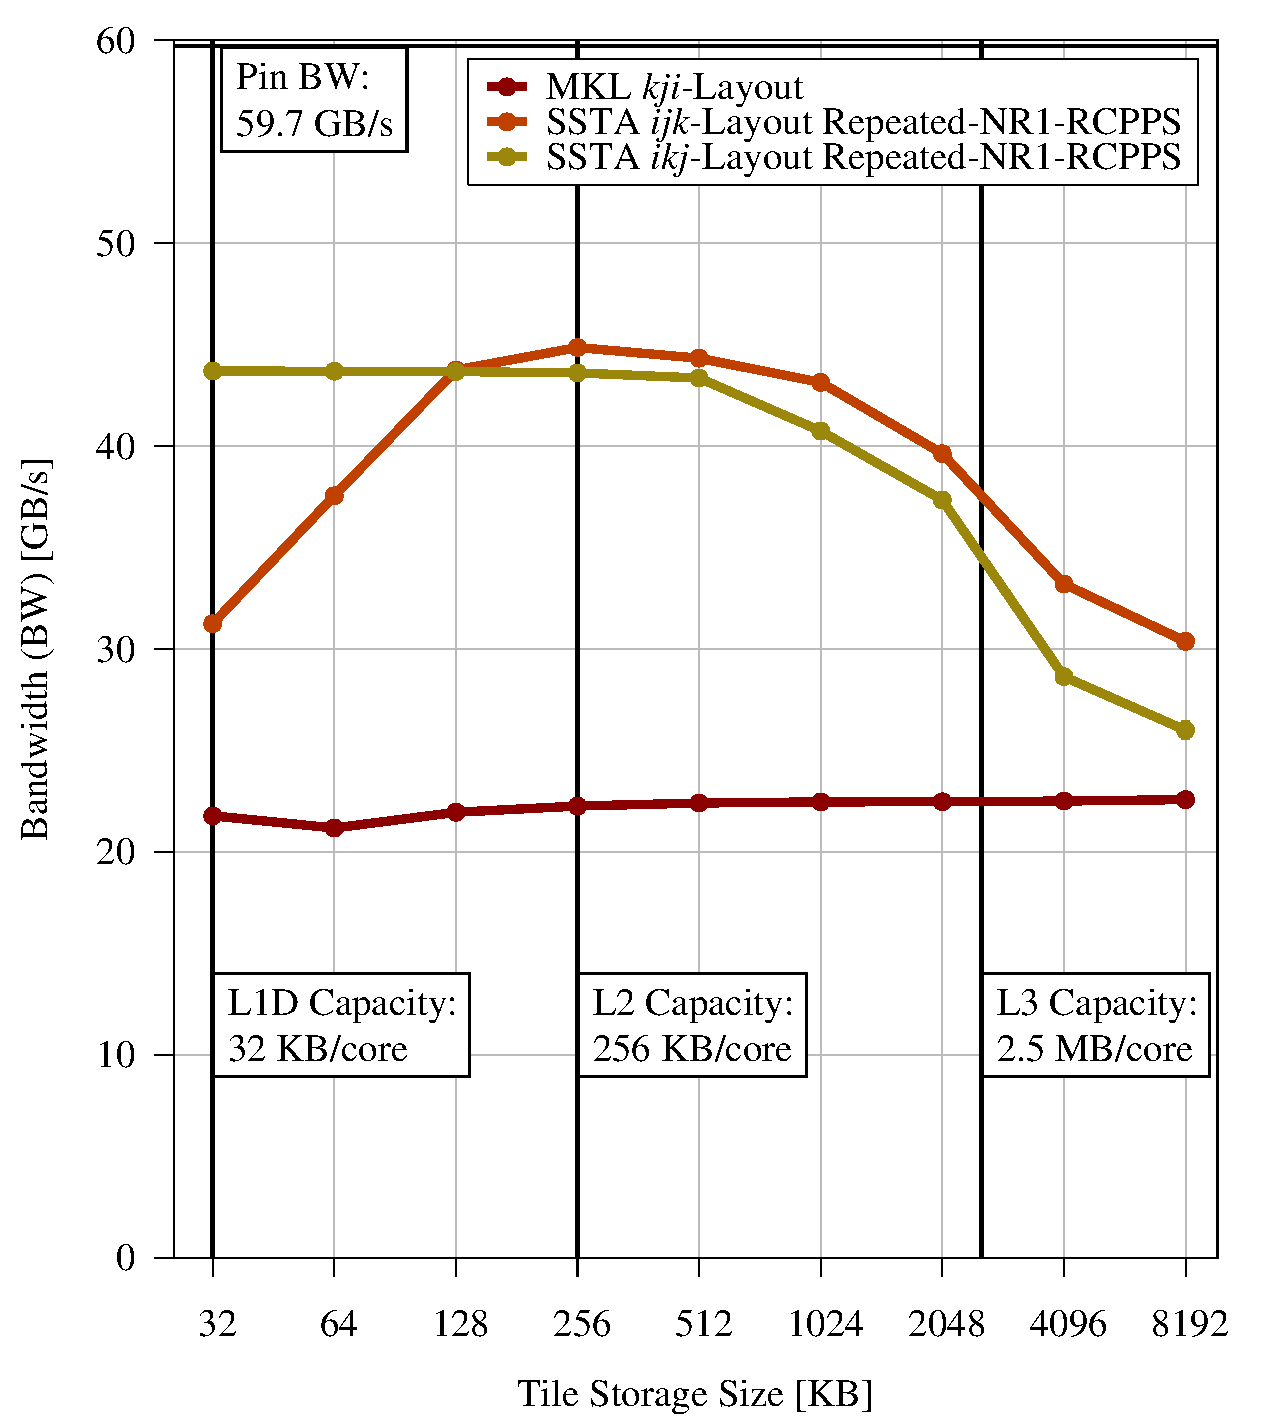
\includegraphics[width=0.99\columnwidth]{figures/post_tsb_tw_sweep_full_matrix_double_precision_production_edison_ivb_e5_2695_v2_08_31_2016_09_03_2016_12pus.pdf}
  \end{minipage}
  \begin{minipage}{0.49\textwidth}
    \centering
    \label{fig:results:tile_size_hsw}
    \caption{
      \textbf{SSTA Total Tile Size vs Effective Bandwidth (Haswell)}
    }
    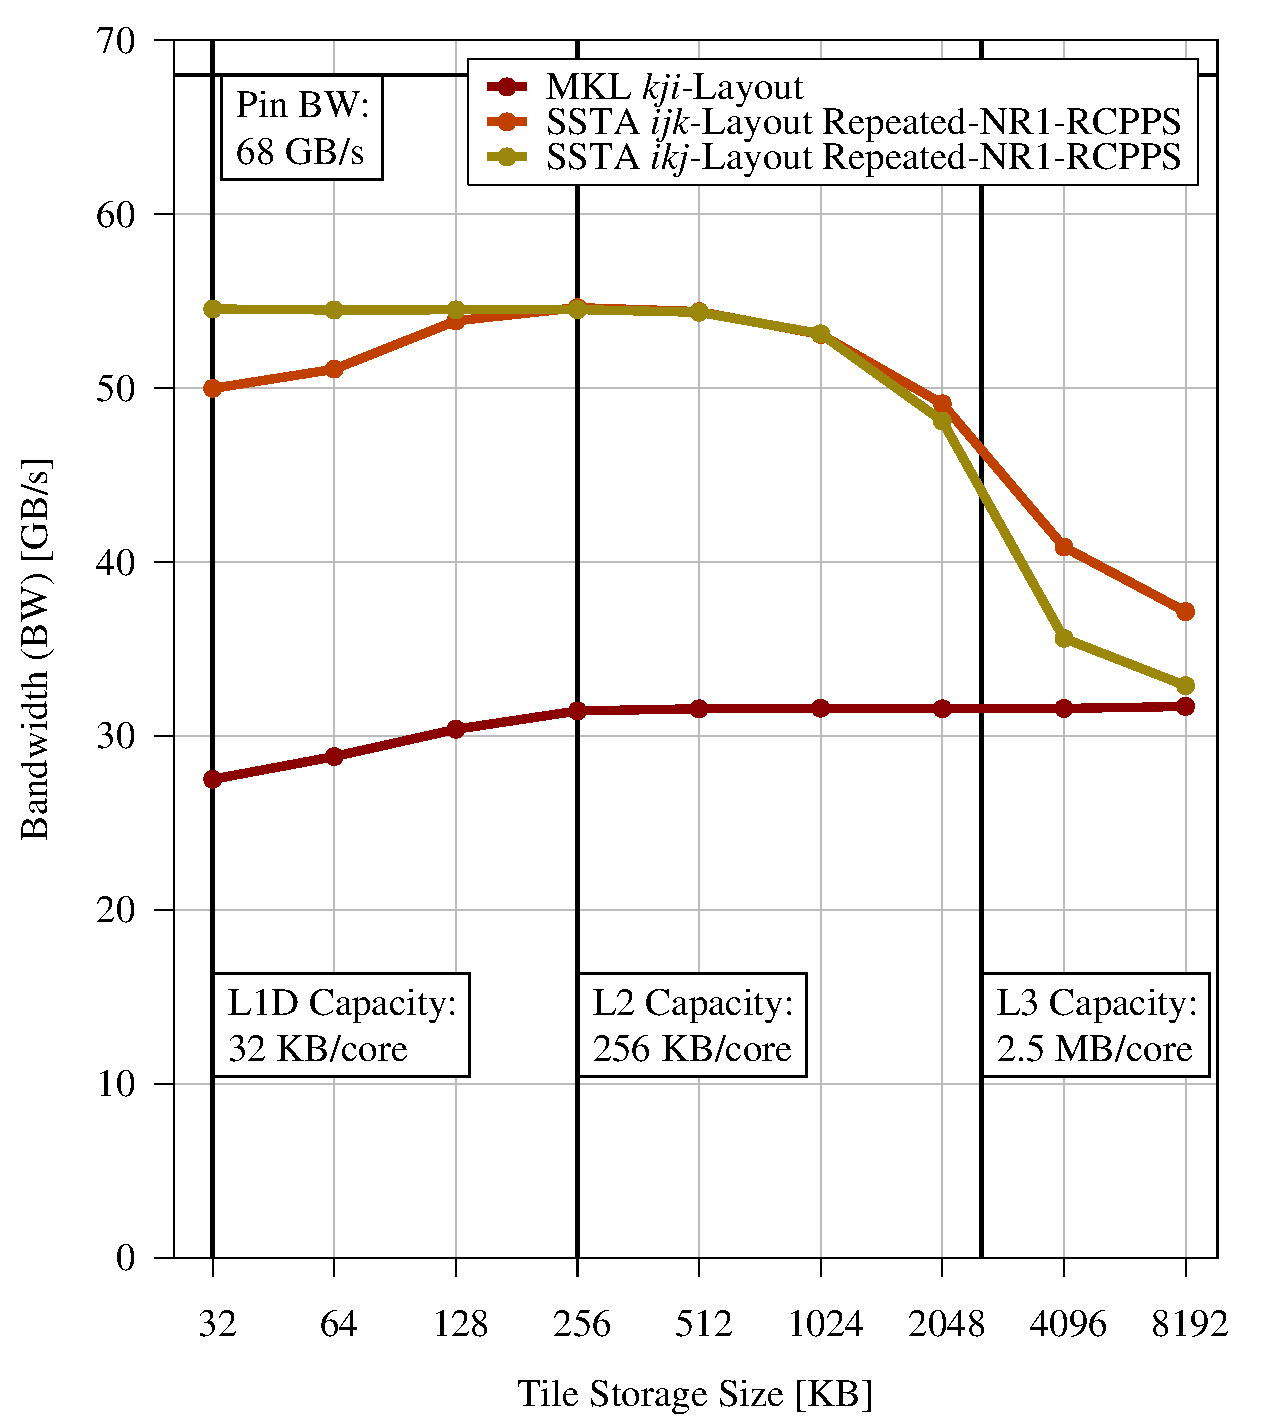
\includegraphics[width=0.99\columnwidth]{figures/post_tsb_tw_sweep_full_matrix_double_precision_production_cori_hsw_e5_2698_v3_08_31_2016_09_03_2016_16pus.pdf}
  \end{minipage}
\end{figure*}

\begin{figure*}[!bth]
  \captionsetup{width=0.39\textwidth}
  \begin{minipage}{0.49\textwidth}
    \centering
    \label{fig:results:tile_size_knl}
    \caption{
      \textbf{SSTA Total Tile Size vs Effective Bandwidth (Knight's Landing)}
    }
    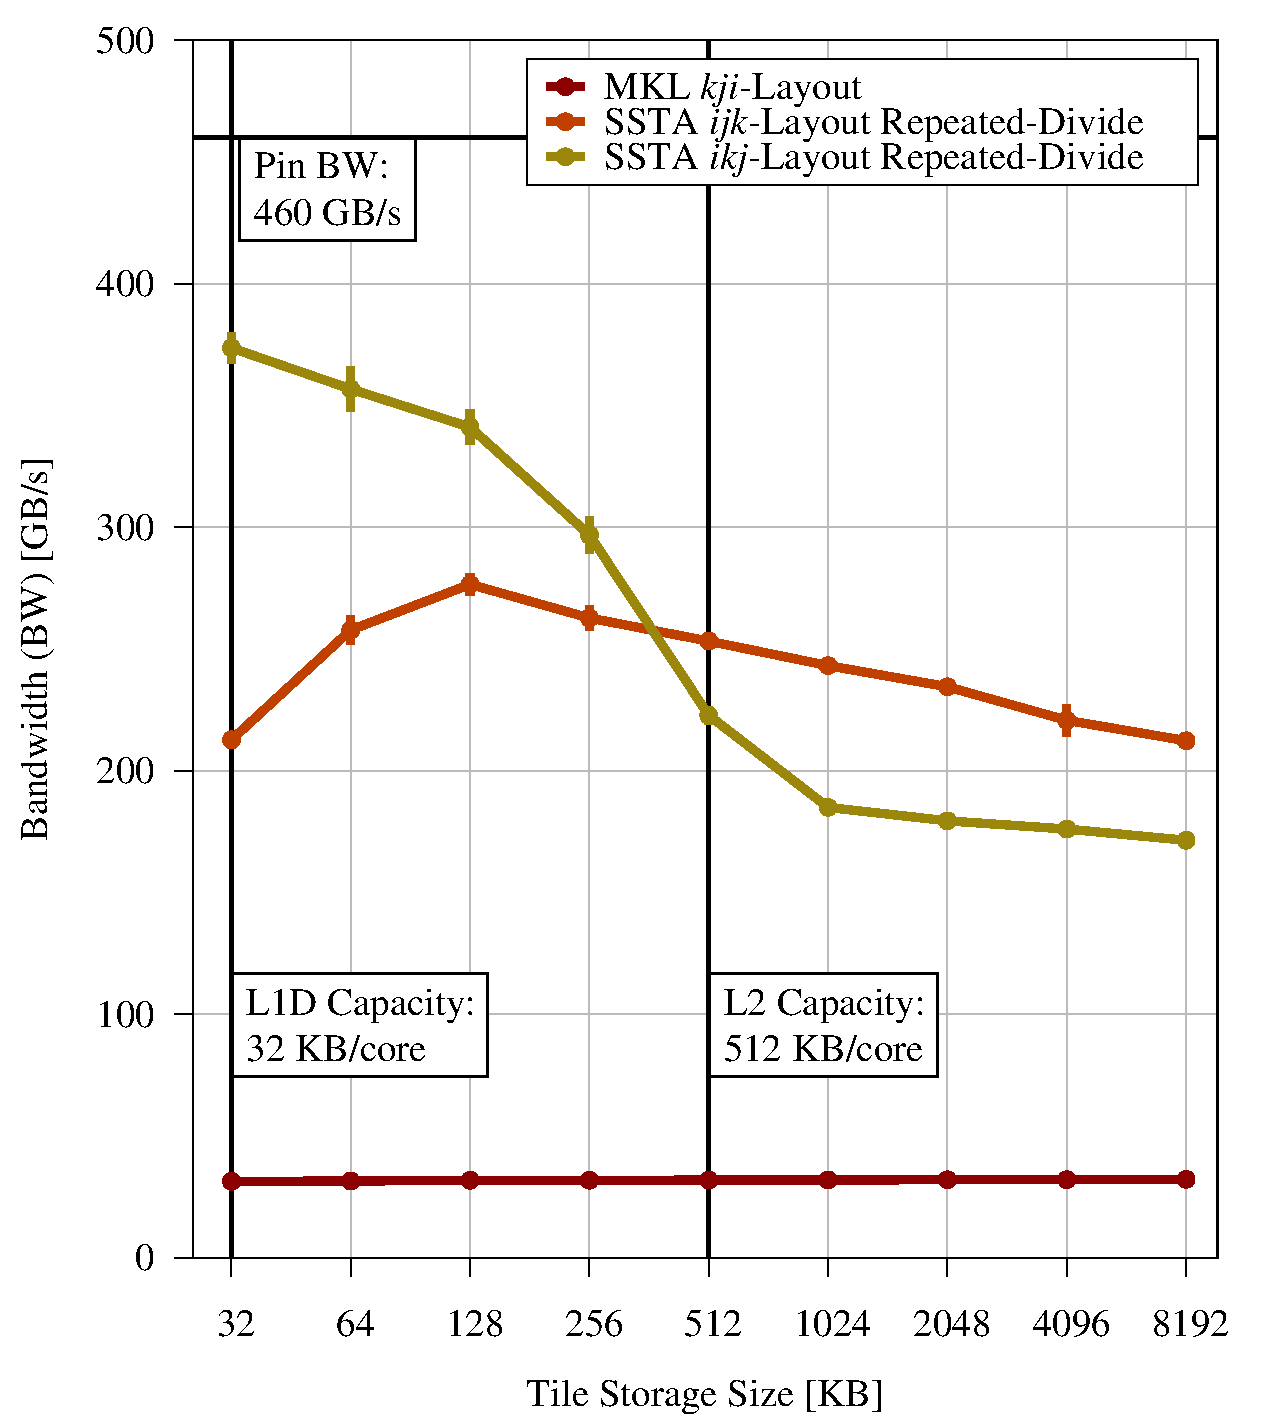
\includegraphics[width=0.95\columnwidth]{figures/post_tsb_tw_sweep_full_matrix_double_precision_production_carl_knl_7210_09_02_2016_64pus.pdf}
  \end{minipage}
  \begin{minipage}{0.49\textwidth}
    \centering
    \label{fig:results:efficiency}
    \caption{
      \textbf{SSTA Efficiency (\% of STREAM Triad Effective Bandwidth)}
    }
    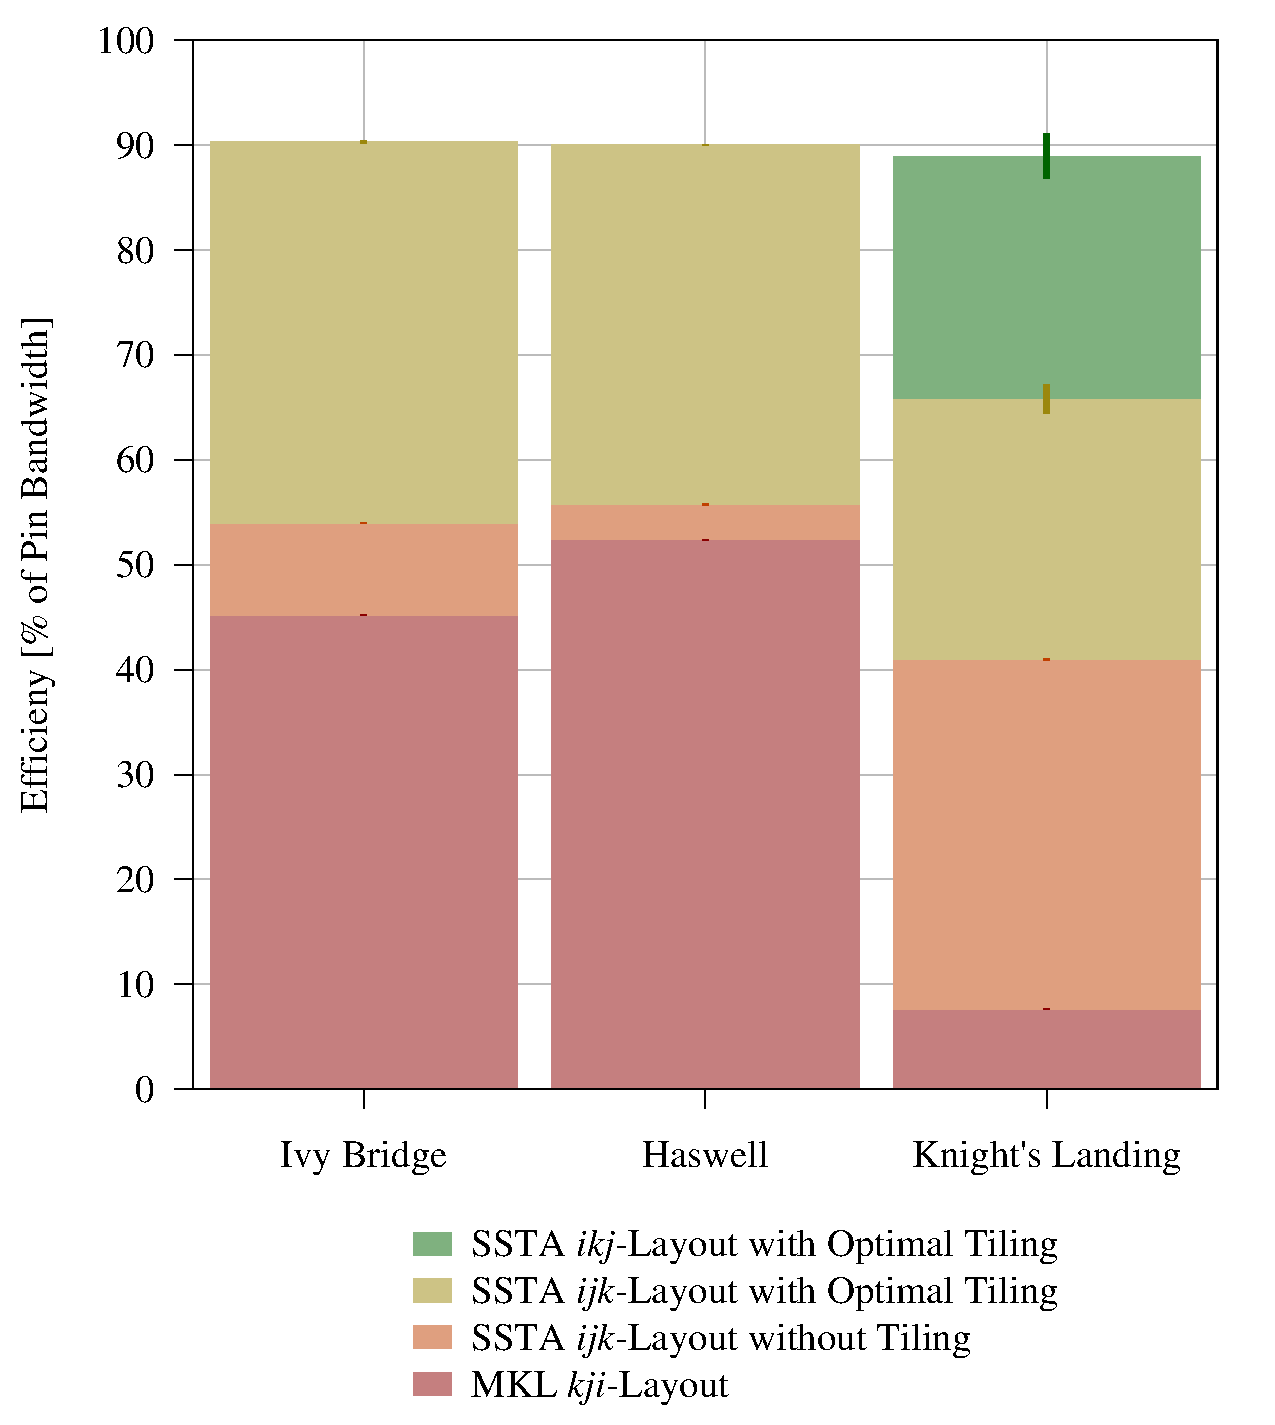
\includegraphics[width=0.95\columnwidth]{figures/post_tsb_impact_of_optimizations_histogram_09_03_2016_09_04_2016_1socket.pdf}
  \end{minipage}
\end{figure*}

% Hypothesis 1.1: SSTA can outperform legacy solver
% Hypothesis 1.2: SSTA can efficiently utilize memory bandwidth 
% Prediction 1.1 and Prediction 1.2 follow naturally 
We developed SSTA to replace the underperforming LAPACK-based vertical column
  solver in our production climate application because we believed that a new
  algorithm which solves multiple vertical columns simultaneously would
  efficiently utilize available memory bandwidth and significantly outperform the
  legacy solver by exhibiting performant data movement patterns and facilitating
  vectorization.

% Hypothesis 2: SSTA will be highly sensitive to total tile size and will
% achieve optimal performance for a particular tile size that balances
% reuse/locality/amortization.
We also theorized that such a solver would be highly sensitive to
  \textbf{total tile size} (\S\ref{sec:implementation:tiling}).
Parallel application performance is often driven by parameters which controls
  the amount of work in each parallel task.
In memory-bandwidth bound applications, these parameters can be especially important
  as they not only control the amount of parallelism exposed but also the working
  set size and degree of cached data reuse in each individual task.
We anticipated that we would need to study the effect of different tile sizes
  in order understand the performance of our new solver and determine the
  \textbf{optimal total tile size}.

The first experiment we performed was a parameter sweep of the total tile size
  on our Xeon and Xeon Phi test platforms.
We predicted that we would see the following: 
\begin{itemize}
% Prediction 2.1
\item Total tile sizes small enough to fit into the L1D cache would not be feasible
  because the overheads of loop constructs, parallelization and vectorization
  would be too great relative to the execution time of useful work per
  inner-iteration.
These tile sizes would either require vertical extents below the sizes used
  by the applications we are interested in (\(nk < 16\)) or horizontal
  dimensions too small to vectorize efficiently (\(ni < 16\)).
% Prediction 2.2
\item The optimal total tile size would fit into the L2 cache (but not the L1D
  cache).
% Prediction 2.3
\item As we move from a tile size which fits into the L2 cache to a tile size
  which does not, we should see a drop in effective bandwidth.
% Prediction 2.4
\item As we move from a tile size which fits into the last level cache (the L3
  cache for the Xeon platforms and the MCDRAM cache for Knight's Landing), we
  should see a drop in effective bandwidth.
% Prediction 2.5
\item Sufficiently large tile sizes should express insufficient parallelism and
  perform poorly due to starvation.
\end{itemize}

The results of this parameter sweep for both the \(ijk\)-layout SSTA variant and
  the \(ikj\)-layout SSTA variant are shown in Figure
  \ref{fig:results:tile_size_ivb} (Ivy Bridge), Figure
  \ref{fig:results:tile_size_hsw} (Haswell) and Figure
  \ref{fig:results:tile_size_knl}.
Results from the TSB suite's MKL baseline solver are shown as a lower bound,
  and STREAM Triad is shown as an upper bound. 
A \(32 \times 147456 \times 32\) grid of double precision floating point values
  was used on all platforms.
The total problem size was 4.5GB.

% Analysis of Prediction 2.1
As we predicted, total tile sizes small enough to fit into the L1D cache were
  impractically small.
% (32KB*1/2*1/4*1/sizeof(double))*(1/nk)*(1/ni)
%       ^^^ ^^^
%        1   2
% 1: reasonable target working set size 
% 2: # of arrays
We would have to either reduce either the vertical extent or the horizontal
  extent \(ni\) to generate a tile size small enough to fit into the 32KB L1D
  with the tile-\(j\) scheme.
We ran preliminary experiments with \(ni=16\) (not shown) to observe the effect
  of 16KB total tile sizes.
The results indicated decreased performance in comparison to \(ni=16\) and
  \(ni=32\) 32KB total tile size results (for \emph{both} data SSTA data layouts).
At \(ni=16\), the trip count on some of the loops in SSTA is so small that the
  compiler cannot perform as much unrolling after vectorization as it would for
  larger \(ni\)s.
\fxnote[footnote,noinline]{Worth mentioning for future work}
We have not determined if switching to the tile-\(ij\) scheme might make
  smaller tile sizes feasible without decreasing the extent of the horizontal
  dimension \(ni\) or decreasing performance via worse data contiguity.

% Analysis of Prediction 2.2
On Knight's Landing, the optimal total tile size for the \(ikj\)-layout is 32KB,
  which fits within the L2 cache but likely does not entirely fit into the L1D
  cache.
We are 95\% confident the effective bandwidth of the SSTA \(ikj\)-layout variant
  is between 364 GB/s and 376 GB/s.

However, on Ivy Bridge and Edison, the optimal tile size for the \(ikj\)-layout
  is between 32KB and 256KB (we cannot statistically distinguish between the results
  as the 95\% confidence intervals overlap).
The 256KB tile size is too large to fit entirely within the L2 cache on these
  platforms as it would require 100\% of the L2 capacity.

% For ijk, the optimal tile size is larger. On KNL, the optimal tile size, 128KB,
% fits within L2 cache. On both Xeon platforms, the optimal tile size is 256KB.
% KNL: The optimal tile size fits within the L2 cache for both layouts. For ijk,
% the best tile size is 128KB. 

% For ijk, performance drops off for smaller tile sizes;
% profiling indicated that this was due to a high number of L1 TLB misses. This
% follows. As discussed in \S\ref{tiling}, tiles in the ijk-layout are made up 
% of nk horizontal ij-planes. As the per-array tile size is decreased, the size
% of the contiguous regions decreases, and reuse of TLB entries decreases.
% We suspect that hardware prefetching is also impacted, especially on KNL. 

% The poor performance of the ijk-layout at smaller tile sizes led us to develop
% the ikj-layout variant of the SSTA algorithm. On the KNL, the ikj-layout had
% the desired effect and substantially increased effective bandwidth.



%We present the results of two experiments which characterize the impact of the
%optimizations described in this paper, support the predictions about optimal
%grain size that we made in Section \ref{} and show how the SSTA algorithm
%performs in comparison with the legacy LAPACK-based approach used in our
%production climate application and the theoretical performance model we
%described in Section \ref{}.
%
%The first experiment is a parameter sweep of different tile sizes. We conducted
%the parameter sweep for all tiled and parallelized TSB variants that were
%feature complete at the time. Although it met those requirements, we excluded
%the MKL variant which uses the kji layout and does gather-style copies of u
%into contiguous buffers to pass to LAPACK. Although it most closely mirrors the
%performance of the original state of the production code, it is not reasonable
%a reasonable reference point because it performs allocations within the timed 
%region.
%
%All variants were used double precision data types, a full grid scheme and
%OpenMP for parallelization. We used a LAPACK-based ijk layout variant which
%uses Intel's MKL library. All the other variants were different instantiations
%of the SSTA algorithm:
%
%%\begin{itemize} 
%%\end{itemize}
%
%Recall that we use the \textbf{tile width} parameter tw (e.g. the j extent of
%the tile) to control the \textbf{tile size} (e.g. the sum of the size of a
%single tile of a, b, c and u). Also recall that we allocate nixnjxnk elements
%instead of nixnjxn(k-1) for the diagonal arrays a and c to simplify our cache
%aliasing conflict mitigation strategy, so the true size of a tile is the
%slightly larger \textbf{tile storage size}, although the extra tile elements
%are never accessed. As described in Section \ref{}, we set ni and nk as 32 for
%this experiment, so the tile storage size will often be a power of 2. To
%simplify visualization, we will use tile storage size instead of tile size or
%tile width in our discussion of this parameter sweep.

%===========================================================================
\section{Conclusion}
\label{sec:conclusion}

We have introduced an approach to maximize throughput and memory
  performance of vectors of different small, tridiagonal matrix solves.
These arise in a number of scientific application contexts, and could
  be an important component of numerical linear algebra libraries.
We have demonstrated that a number of trade-offs exist: between tile size,
  data layout, vectorization features (division, reciprocal, etc.),
  and constraints from the memory hierarchy.
For pre-KNL architectures, we have shown some benefit from an iterative
  single-precision inverse that reduces instruction latency for divides; 
  for the KNL architecture that supports vectorized divides, 
  there was little benefit.
Across all architectures, the benefit in VTDMA was evident from 
  memory bandwidth, with improvements over single-matrix MKL ranging 
  from \fxnote{$XX\%$} of pin bandwidth for IVB and HSW to 
  \fxnote{$XX\%$} on KNL.
The sensitivity to tile size clearly showed that L1, L2, and TLB effects
  need to be considered carefully when exploring the optimization space.
Changing data layouts between natural \(ijk\) indices and \(kij\) 
  or \(ikj\) made a substantial difference in performance, 
  and it was determined that \(ikj\) provides the best 
  \fxnote{$XX\%$} improvement.
Overall, the difference between a naive loop and MKL implementation,
  and one optimized for vectorization and memory hierarchy on KNL 
  can be as much as \fxnote{$XX\%$}.

\section{Future Work}
\label{sec:future_work}

A number of possible research directions are possible from VTDMA.
The existing algorithm is directly applicable to block-tridiagonal matrices,
  where diagonal and off-diagonal blocks can be solved simultaneously
  to accelerate larger, distributed matrix solves.
This would also be the basis for better strong scaling by tiling in
  the vertical $k$ direction as well, and potentially smaller
  tile sizes overall. 
The current algorithm needs to be extended to include matrix assembly
  based on solution values, and put inside a fully non-linear iteration
  with a Jacobian calculation, such as used in Newton iterations;
  the challenge here is that some columns may converge faster than
  others, and vector masks or scalar iterative refinement may be required.
Opportunities to extend the algorithm to banded matrices and ILU-type 
  algorithms are straight-forward for diagonally-dominant cases, but
  pivoting has the potential to hinder vectorization if not carefully
  implemented.
Finally, a more complex application would involve other operations,
  such as traditional ``stencil'' finite difference operations and
  time integration algorithms; it remains to be seen if there are
  performance trade-offs between \(ijk\) and \(ikj\) in 
  these applications.
This is particularly important for unstructured mesh applications,
  where mesh partitioning usually provide only \(ik\) 
  data alignment to applications.

\fxnote{Bryce: Sentence about rolling matrix?}

% Need a section explaining tile size / tile storage size

% Future work should mention smaller tile sizes.

%===========================================================================
%\section*{Acknowledgments}
%
%This material is based upon work supported by the U.S. Department of Energy, Office of Science, Advanced Scientific Computing Research, Scientific Discovery through Advanced Computing (SciDAC) program.
%This work was partially supported by the Intel Parallel Computing Center at
%Lawrence Berkeley National Laboratory,
%and used resources at the National Energy Research Scientific Computing Center, which are supported by the U.S. Department of Energy Office of Science's Advanced Scientific Computing Research program under contract number DE-AC02-05CH11231.  
%This research used resources in Louisiana State University's Center for Computation and Technology. 
%\fxnote{Bryce: Check with Adrian if there's wording here that LSU likes}

%This research used resources of the National Energy Research Scientific Computing Center (NERSC), which is supported by the Office of Science of the U.S. Department of Energy under contract DE-AC02-05CH11231.
%This research used resources of the Argonne Leadership Computing Facility at Argonne National Laboratory, which is supported by the Office of Science of the U.S. Department of Energy under contract DE-AC02-06CH11357.
%This research used resources of the Oak Ridge Leadership Facility at the Oak Ridge National Laboratory, which is supported by the Office of Science of the U.S. Department of Energy under Contract No. DE-AC05-00OR22725.


%===========================================================================
\bibliographystyle{IEEEtran}
\bibliography{sc16-implicit}
%===========================================================================

%===========================================================================
% 

%\section*{Notes/Outline}
%Submission info:
%\url{https://easychair.org/conferences/?conf=pmbs16}
%
%\begin{itemize}
%\item Climate apps use HE-VI model 3D+1D. Also a pattern for 2D+1D and 3D+0D chemistry
%\item Results demonstrate importance of ``batching'' solves, MLK doesn't do
%\item Cache coherency is important: IMEX RK accum, tiling
%\item Explicit part is HO stencil op, memory b/w bound (w/ ghost cells)
%\item Implicit part is non-linear solver: App requires different matrix at each i,j index 
%\item Results in repeated vertical sparse banded solve
%\item Solve (tridiag, banded, dense) should vectorize on i (unit stride), tiled in pencils
%\item Considerations for vector alignment, tiling, and memory
%\item Performance results, scaling, comparison, by platform / parameter
%\item Future work: communication hiding, load imbalance, IMEX
%\end{itemize}
%(Bryce's email comments) Looking over the outline:
%\\
%It's crucial that we clearly identify the optimizations that we
%believe are novel/high-impact, vs the optimizations that are
%well-known to the community (even if they were not well known to us).
%For example, on the outline, we have listed "IMEX RK accum, tiling".
%Do we want to present the accumulation optimizations which removed
%unnecessary temporaries from the time integrator? Do we feel that
%optimization is novel, or is that just a common-sense thing that only
%affected us because of the Chombo programming model? Likewise, do we
%want to present tiling as a focal point in this paper? Tiling is a
%well-known technique; we certainly can't claim tiling in general as
%novel work. Is some part of our tiling approach novel? (how about
%parallelizing the tile loop - is that fairly novel? I know Sam does
%this in HPGMG, but is this a widely used technique?)
%\\
%We would be well served by applying the scientific method at this juncture:
%\\
%\begin{itemize}
%\item Question: What concrete research question(s) are we answering?
%\begin{itemize}
%\item Prior research indicates that HE-VI methods show promise as a
%scalable approach to solving global climate problems on cubed sphere
%geometries because <explanation> [cite prior studies]. How do we
%implement HE-VI methods which perform well on cache-coherent SIMD
%architectures?
%\item When solving a problem with a high horizontal-vertical aspect ratio
%(e.g. the horizontal extents are much greater than the vertical
%extents) with HE-VI methods, it is necessary to perform a large number
%of small vertical implicit solves (<give examples of matrix sizes>
%[citation]) which are independent of each other. <explain the type of
%solves in the climate dycore - e.g. non-linear but nearly banded>
%[citation]. How can we efficiently solve large quantities of small
%non-linear bandedish/banded/tridiagonal matrices on cache-coherent
%SIMD architectures?
%\end{itemize}
%\item Hypothesis: What theories did we come up with that would answer our
%research question(s)?
%\begin{itemize}
%\item Optimal memory access patterns, management of working set sizes
%(e.g. staying in cache) and efficient use of vector units are
%necessary to achieve good performance on cache-coherent SIMD
%architectures.
%\begin{itemize}
%\item Optimal memory access patterns: moving through memory in unit
%stride, controlling the number of streams.
%\item Management of working set sizes: tiling, reducing size of
%temporaries/localizing temporaries (thread-local or otherwise)
%\item Efficient use of vector units: moving through memory in unit
%stride, controlling memory alignment, controlling array strides,
%annotation-assisted autovectorization
%\item TODO: List of individual, concrete optimizations from above.
%\end{itemize}
%\item Mainstream linear algebra libraries (<examples> [citation]) are not
%well-suited for solving large quantities of small non-linear
%bandedish/banded/tridiagonal matrices on cache-coherent SIMD
%architectures because <expalanation> [cite prior studies if possible].
%\end{itemize}
%
%
%\item Prediction: If our hypotheses are true, what results can we expect to
%see? \\
%$\rightarrow$ TODO: What performance characteristics should we see with and
%without each of the concrete optimizations from our hypothesis above?
%
%\item Experiment: Investigate the predictions we've made. \\
%$\rightarrow$ TODO: Methodology for benchmarking the optimizations identified
%above and measuring the performance characteristics we're interested
%in.
%
%\item Analysis: What were the results of our experiments?
%\end{itemize}
%
%List of figures from meeting on 8/11:
%For KNL, HSW, SNB(?)...
%List of figures from meeting on 8/11:
%-For KNL, HSW, SNB(?)...
%\begin{enumerate}
%\item Baseline performance using MKL (and hand) using i-major data layout 
%(not vectorized)
%\item Performance as a function of 32b RCP NR (not needed on KNL), stored
%reciprocal (cuts divides in half) for fixed file size (4?)
%\item Performance vs. Tile Size (jtile = 1,2,4,8,16,32)
%\item Best Performance vs. MKL using same data layout vs. MKL using its best
%(include DRAM BW limit)
%\item Performance as a function of total parallelism for constant tile size
%[optional time permitting]
%\item Performance with 2,3,4 hyperthreads...  maybe just prose comments?
%\item effect of kdim != pow(2)... maybe just prose comments?
%\end{enumerate}
\newpage
\section*{TODO}

\fxnote{from SAM: I think the paper/abstract should respond to a few points in 
their topics of interest...}
\begin{itemize}
\item Performance evaluation and lessons learnt \\
  == Early/First examination of KNL for climate codes
\item Extensions to and shortcomings of current accelerator directives APIs \\
  == some comment on observation that compilers are unable to see beyond OMP on
a column and realize a loop transformations (for vectorization) across multiple
columns can be performed.
\item Auto-tuning and optimization strategies \\
  == tuning tile sizes / caching divides / etc...
\end{itemize}

\fxnote{HANS: Most of the length is due to two competing goals for the paper: 
  an optimization process, or a benchmark. Skip the benchmark for now \dots}

\fxnote{SAM/HANS: is anything learned from single-core results here? Drop?}

\fxnote{HANS: where is the discussion of how the B/W is calculated? 
  Where are the wallclock times?}


\begin{figure*}
\listoffixmes
\end{figure*}

\end{document}


